\documentclass{article}

% =========================================================================
% COLLABORATION MARKUP TOGGLE:
%   \markchangestrue  -> highlights inline edits (\dmedit) in dark red and
%                        frames new review blocks/figures in red boxes.
%   \markchangesfalse -> renders an unmarked black manuscript PDF.
% =========================================================================
\newif\ifmarkchanges
\markchangestrue

\usepackage{arxiv}

\usepackage[utf8]{inputenc}
\usepackage[T1]{fontenc}
\usepackage{xcolor}
\usepackage[colorlinks=true, allcolors=blue!70!black]{hyperref}
\usepackage{url}
\usepackage{booktabs}
\usepackage{amsfonts}
\usepackage{nicefrac}
\usepackage{microtype}
\usepackage{graphicx}
\graphicspath{ {./images/}{./} }
\setlength{\marginparwidth}{2cm}
\usepackage{todonotes}
\usepackage{subcaption}
\usepackage{lineno}
\usepackage{tikz}
\usetikzlibrary{arrows.meta, positioning}
\linenumbers
\usepackage{amsmath}
\usepackage{amssymb}
\usepackage{multirow}
\usepackage{array}
\usepackage{dmmarkup}

\title{Self-Supervised Representation Learning on Full-Event Collider Tracks: Tokenisation, Augmentation Geometry, and Calibrated Anomaly Detection}

\author{
 Aritra Das \\
  Department of Physical Sciences\\
  IISER Kolkata\\
  Kolkata \\
  \texttt{\href{mailto:ad21ms061@iiserkol.ac.in}{ad21ms061@iiserkol.ac.in}} \\
   \And
 Daniel Thomas Murnane \\
  Niels Bohr Institute\\
  University of Copenhagen\\
  Copenhagen \\
  \texttt{\href{mailto:daniel.murnane@nbi.ku.dk}{daniel.murnane@nbi.ku.dk}} \\
  \And
 Shreya Saha \\
  School of Physics, Chemistry and Earth Sciences\\
  Adelaide University\\
  Adelaide \\
  \texttt{\href{mailto:shreya.saha@adelaide.edu.au}{shreya.saha@adelaide.edu.au}} \\
}

\begin{document}
\emergencystretch=1.5em
\maketitle

\begin{abstract}
General-purpose representations of full-event charged-particle track collections offer a practical route toward reusable event encoders at the High-Luminosity Large Hadron Collider. Designing self-supervised objectives for variable-length sets of helical trajectories raises three concrete questions: whether discrete vector-quantised track tokenisers match continuous set encoders and deterministic physics summaries across bottleneck dimensions, how kinematically consistent coordinate augmentations shape contrastive embeddings, and whether representations that maximise Standard Model classification also maximise discovery power in signal-agnostic goodness-of-fit testing. Holding the permutation-invariant Set Transformer architecture fixed across set-level pretraining objectives, we benchmark 27 primary track-level representations alongside end-to-end supervised and fine-tuned baselines on $1.85\times 10^6$ zero-pileup simulated proton-proton collisions from ColliderML, partitioned without overlap into $900,000$ Standard Model pretraining events and $950,000$ downstream evaluation events. Kinematically consistent continuous contrastive pretraining reaches $68.0\%$ three-class Standard Model linear probe accuracy at $D=64$, and contrastive pretraining over an $8192$-code contextual vector-quantised track tokeniser reaches $68.9\%$, both outperforming deterministic 28-feature track summaries on linear classification and improving low-label accuracy at $100$ to $1,000$ labelled events under two-stage fine-tuning. The $8192$-code tokeniser uses $100\%$ of its codebook on Standard Model tracks, retains $97.5\%$ threshold recall on reconstructed displaced tracks with $|d_0| > 1\text{ mm}$, and yields matching downstream performance before and after quantisation. Using empirically calibrated Kernel New Physics Learning Machine tests ($10,000$ background toys per representative model), multiplicity reweighting, impact-parameter masking, and covariance whitening, we uncover a sharp task-metric trade-off: supervised Standard Model encoders concentrate variance into a low-rank subspace ($\text{erank}_{\text{SM}} \le 3.5$), leading Standard Model classification and Hidden Valley dark-shower detection while losing high-purity tail recall on displaced Higgs Portal decays, where compact tail-preserving embeddings ($D=8$ vector-quantised poolings and a six-observable displaced-track baseline) achieve two- to eightfold higher anomaly sensitivity.
\end{abstract}

\section{Introduction}
\label{sec:intro}

High-luminosity proton-proton collisions at the Large Hadron Collider motivate general-purpose event representations that map variable-length particle sets into reusable latent spaces~\cite{JetCLR,ResimulationSSL,OmniJetAlpha,OmniLearn,MPM,BinnedTokenizationHEP}. Whereas jet-level foundation models operate on tens of constituents confined within a single jet cone~\cite{ParT,OmniJetAlpha,OmniLearn,MPM}, full-event inner-detector collections contain up to several hundred helical trajectories spanning multiple jets and displaced decay vertices. Extending self-supervised representation learning to full-event tracking raises three methodological questions:
\begin{enumerate}
    \item \emph{Continuous versus discrete track encodings.} Reconstructed perigee parameters span several orders of magnitude, from sub-millimetre transverse impact parameters tagging long-lived particle decays to multi-hundred-GeV momenta. Discretising tracks with a Vector-Quantised Variational Autoencoder (VQ-VAE)~\cite{VQVAE} enables token-based pretraining, provided that a codebook fit exclusively on Standard Model (SM) events preserves out-of-distribution displaced-track tails.
    \item \emph{Contrastive augmentation geometry under a fixed backbone.} Comparing pretraining paradigms fairly requires holding the encoder architecture fixed so that downstream differences reflect the objective and bottleneck dimension rather than model capacity. In SimCLR-style contrastive pretraining~\cite{SimCLR,JetCLR}, positive-pair perturbations must also respect perigee kinematic identities such as $p_T = p\sin\theta$ while perturbing per-track polar and azimuthal angles so a permutation-invariant Set Transformer~\cite{SetTransformer} cannot exploit trivial angular invariants.
    \item \emph{Supervised separability versus kernel goodness-of-fit discovery.} Pretrained collider embeddings are intended both for supervised transfer classification and for signal-agnostic two-sample testing with the New Physics Learning Machine (NPLM)~\cite{NPLM2019,NPLM2021,KernelNPLM2022,NPLMEmbedding2025}. Whether representations optimised for SM process separation outperform compact reconstruction bottlenecks or classical collider observables under isotropic kernel testing remains an empirical question.
\end{enumerate}

We investigate these questions through a controlled benchmark on ColliderML Release 1~\cite{ColliderML,ColliderMLDataset} at zero pileup ($\langle\mu\rangle = 0$). Pretraining uses $900,000$ unlabelled SM events, and downstream evaluation uses a disjoint $950,000$-event sample spanning three SM processes and two Beyond-the-Standard-Model (BSM) benchmarks: a long-lived Higgs Portal scalar decaying to displaced $b$-jets and a confining Hidden Valley dark shower~\cite{StrasslerZurek2007}. Across 27 primary representations, from-scratch supervised baselines, and fine-tuned encoders, our main findings are:
\begin{itemize}
    \item Holding the Pre-LN Set Transformer backbone fixed across set-level objectives, kinematically consistent continuous contrastive pretraining reaches $68.0\%$ three-class SM linear accuracy at $D=64$, and tokenised contrastive pretraining over an $8192$-code contextual VQ-VAE reaches $68.9\%$. Combined with two-stage linear-probe-then-fine-tuning (LP-FT)~\cite{LPFT2022}, unlabelled pretraining improves accuracy and reduces seed variance by six- to tenfold at $100$ to $1,000$ labelled events.
    \item Fitted solely on SM tracks, the $8192$-code contextual VQ-VAE achieves $100\%$ codebook utilisation, retains $97.5\%$ threshold recall on reconstructed displaced tracks with $|d_0| > 1\text{ mm}$, and agrees within $0.0023$ across all probe metrics before and after vector quantisation.
    \item Using a double-precision GPU Newton-Raphson solver for Falkon kernel logistic regression~\cite{KernelNPLM2022}, we calibrate exact order-statistic thresholds on $10,000$ held-out background toys per representative model while isolating kinematic shape sensitivity from overall event-rate excesses.
    \item Model rankings invert between supervised probes and signal-agnostic anomaly detection. Supervised SM contrastive embeddings achieve $0.941$ binary transfer ROC-AUC on displaced Higgs Portal decays and lead Hidden Valley detection ($\text{SNR}_{1\%} = 35.0$), yet drop to $\text{SNR}_{1\%} = 3.6$ on Higgs Portal. Using extreme-tail ROC analysis down to $\text{FPR} = 10^{-4}$, impact-parameter masking, and ZCA whitening, we show that SM-class clustering sacrifices high-purity tail recall between SM lobes while isotropic Euclidean kernels reward compact tail-preserving spaces ($D=8$ VQ-VAE poolings at $\text{SNR}_{1\%} = 17.1$, and a six-observable displaced-track baseline at $\text{SNR}_{1\%} = 28.0$).
\end{itemize}

Related work is reviewed in Section~\ref{sec:related}. In Section~\ref{sec:dataset} we describe the ColliderML samples, track parameterisations, and zero-leakage data split. In Section~\ref{sec:rep_learn} we define the unified Set Transformer backbone, pretraining objectives, and physics baselines. In Section~\ref{sec:validation} we evaluate latent effective rank, downstream linear probes, and low-label fine-tuning. In Section~\ref{sec:nplm} we present calibrated Kernel NPLM anomaly detection, mechanistic tracking and kernel-geometry controls, and sensitivity scaling relative to LHC exclusion limits. Conclusions follow in Section~\ref{sec:conclusion}, with full architectural tables, probe sweeps, and calibration diagnostics in Appendices~\ref{app:arch} to~\ref{app:lowd_sweep}.

\section{Related Work}
\label{sec:related}

\paragraph{Self-supervised collider representations.}
Contrastive learning on particle sets was introduced in JetCLR~\cite{JetCLR}, applying SimCLR~\cite{SimCLR} to jet constituents via rotational symmetries and soft-collinear augmentations. Re-simulation positive pairs in RS3L grounded contrastive views in parton-shower and detector stochasticity~\cite{ResimulationSSL}, alongside supervised permutation-equivariant architectures such as Particle Transformer~\cite{ParT}. Discrete jet tokenisation and masked particle modelling have enabled multi-task jet foundation models including binned and VQ-VAE jet tokenisers~\cite{BinnedTokenizationHEP}, OmniJet-$\alpha$~\cite{OmniJetAlpha}, OmniLearn~\cite{OmniLearn}, and Masked Particle Modeling~\cite{MPM}. Whereas jet studies focus on four-momenta within single cones, we examine full-event reconstructed track sets in a $3.0\text{ T}$ solenoidal field where perigee impact parameters encode macroscopic decay lengths.

\paragraph{Kernel goodness-of-fit anomaly detection.}
The New Physics Learning Machine formulates model-independent anomaly detection as an extended log-likelihood ratio test between a reference background sample $\mathcal{R}$ and experimental data $\mathcal{D}$~\cite{NPLM2019,NPLM2021}. Nystr\"om kernel logistic regression improved statistical regularity and computational speed~\cite{KernelNPLM2022,Wilks1938}, with recent extensions introducing multiple-testing aggregation across kernel bandwidths~\cite{GrossoLetizia2024} and goodness-of-fit testing directly on pretrained collider embeddings~\cite{NPLMEmbedding2025}. Building on this framework, we benchmark 23 neural representations alongside four deterministic physics baselines on identical event draws, separate Poisson yield and track-multiplicity shifts from impact-parameter shape information, and connect kernel discovery power to extreme low-false-positive-rate ROC tails.

\section{ColliderML Dataset and Track Representation}
\label{sec:dataset}

ColliderML Release 1~\cite{ColliderML,ColliderMLDataset} provides full detector simulation and reconstruction of $\sqrt{s} = 14\text{ TeV}$ proton-proton collisions in the OpenDataDetector geometry ($3.0\text{ T}$ solenoidal magnetic field). Throughout this work we analyse the zero-pileup (\texttt{pu0}, $\langle\mu\rangle = 0$) configuration so that hard-scatter and displaced-vertex representations can be isolated without pileup-mitigation confounds. Events are generated with \textsc{Pythia}~8.3~\cite{Pythia83}, propagated through \textsc{Geant4}~\cite{Geant4} within \textsc{DD4hep} preserving macroscopic long-lived decay vertices above $1\,\mu\text{m}$, digitised, and reconstructed into helical tracks via \textsc{ACTS}~\cite{ACTS}:

\begin{center}
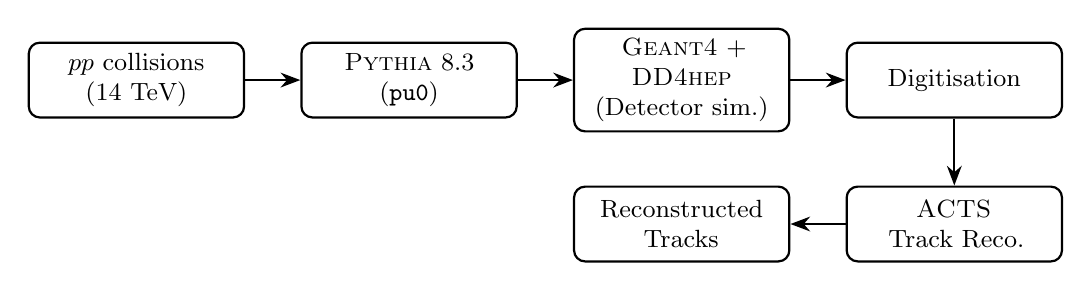
\begin{tikzpicture}[
    node distance=0.6cm and 0.7cm,
    box/.style={
    rectangle, draw, thick, rounded corners,
    minimum height=0.95cm, text centered,
    text width=2.5cm, font=\small
    },
    arr/.style={-{Stealth[length=2.5mm]}, thick}
]
\node[box] (pp) {$pp$ collisions\\($14\text{ TeV}$)};
\node[box, right=of pp] (pythia) {\textsc{Pythia}~8.3\\(\texttt{pu0})};
\node[box, right=of pythia] (geant) {\textsc{Geant4} + \textsc{DD4hep} \\ (Detector sim.)};
\node[box, right=of geant] (digi) {Digitisation};
\node[box, below=0.85cm of digi] (acts) {\textsc{ACTS} \\ Track Reco.};
\node[box, left=of acts] (tracks) {Reconstructed Tracks};

\path[arr] (pp) edge (pythia);
\path[arr] (pythia) edge (geant);
\path[arr] (geant) edge (digi);
\path[arr] (digi) edge (acts);
\path[arr] (acts) edge (tracks);
\end{tikzpicture}
\end{center}

We study three SM background channels ($t\bar{t}$, gluon-gluon fusion single-Higgs production $\text{ggF } H$, and non-resonant di-Higgs production $HH$, decayed inclusively according to SM branching ratios) alongside two BSM signal benchmarks steered with exclusive decays:
\begin{itemize}
    \item \emph{Displaced Higgs Portal (\texttt{HiggsBSM:gg2H2 = on}).} A resonant $125\text{ GeV}$ scalar decays into a pair of neutral long-lived pseudoscalars ($H \to A_0 A_0$), each decaying exclusively to $b\bar{b}$ with mass $m_{A_0} = 55\text{ GeV}$ and proper decay length $c\tau_0 = 100\text{ mm}$. As shown in Fig.~\ref{fig:dataset_dists}, $7.91\%$ of reconstructed tracks satisfy $|d_0| > 1\text{ mm}$ (versus $3.66\%$ in the combined SM sample), while mean track multiplicity drops from $52.2$ to $38.1$ because standard \textsc{ACTS} inside-out pixel seeding loses efficiency for decays occurring beyond the inner pixel layers~\cite{ATLASLRT2023}.
    \item \emph{Hidden Valley dark shower (\texttt{HiddenValley:gg2DvDvbar = on})~\cite{StrasslerZurek2007}.} Pair-produced dark quarks shower in a confining $SU(3)_v$ sector with confinement scale $\Lambda_v = 40\text{ GeV}$ and radiation cutoff $44\text{ GeV}$, yielding invisible $10\text{ GeV}$ diagonal dark pions alongside prompt off-diagonal $10\text{ GeV}$ pions and $20\text{ GeV}$ vector mesons that hadronise into high-multiplicity semi-visible SM jets.
\end{itemize}

\begin{figure}[t]
    \centering
    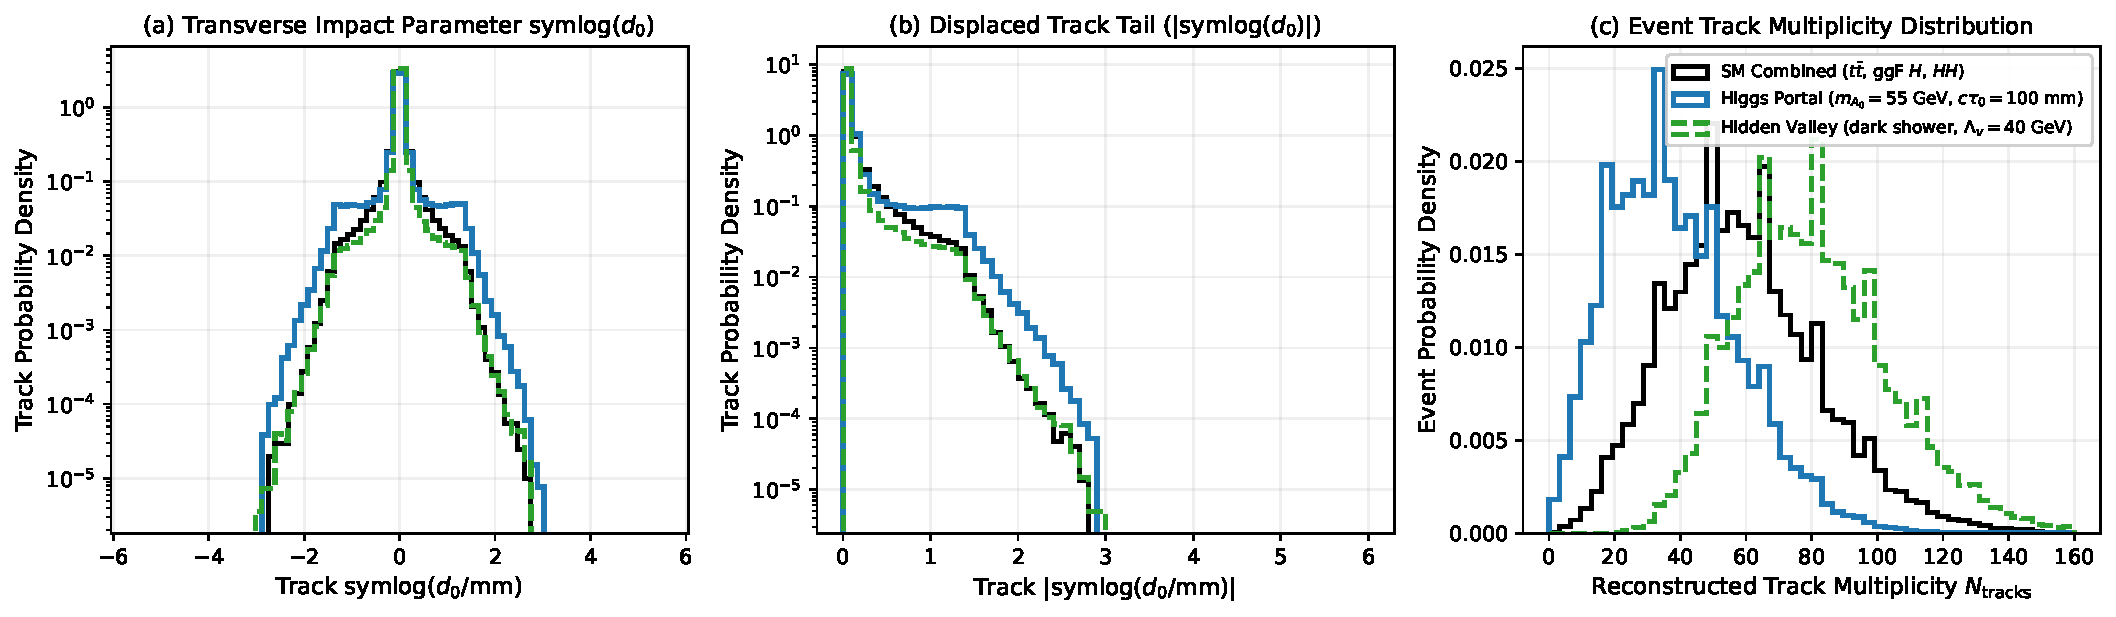
\includegraphics[width=0.97\textwidth]{fig_dataset_distributions.pdf}
    \caption{Track impact-parameter and event multiplicity distributions across held-out Standard Model events (solid black), displaced Higgs Portal decays ($m_{A_0} = 55\text{ GeV}$, $c\tau_0 = 100\text{ mm}$, solid blue), and Hidden Valley dark showers ($\Lambda_v = 40\text{ GeV}$, dashed green): (a) signed $\text{symlog}(d_0/\text{mm})$, (b) $|\text{symlog}(d_0/\text{mm})|$, and (c) reconstructed track multiplicity $N_{\text{tracks}}$.}
    \label{fig:dataset_dists}
\end{figure}

Each reconstructed track is specified by its transverse and longitudinal perigee impact parameters $(d_0, z_0)$, momentum magnitude $p$, transverse momentum $p_T$, polar angle $\theta$, and azimuthal angle $\phi$. Replacing $(\theta, \phi)$ with continuous Cartesian direction cosines $(t_x, t_y, t_z) = (\cos\phi\sin\theta, \sin\phi\sin\theta, \cos\theta)$ avoids azimuthal branch cuts, and applying $\text{symlog}(x) = \text{sign}(x)\ln(1 + |x/\text{mm}|)$ compresses heavy impact-parameter tails while preserving sign. Sorting tracks within each event $i$ by descending $p_T$ up to a cap of $T$ tracks ($T = 128$ in the unified backbone) gives the seven-feature continuous track representation
\begin{equation}
    \mathbf{x}_{ij} = \big(\text{symlog}(d_{0,ij}),\, \text{symlog}(z_{0,ij}),\, p_{ij},\, p_{T,ij},\, t_{x,ij},\, t_{y,ij},\, t_{z,ij}\big) \in \mathbb{R}^7 .
    \label{eq:track_vec7}
\end{equation}
For the contextual VQ-VAE tokeniser, each track is expressed in cylindrical coordinates relative to the leading-$p_T$ track azimuth $\phi_{i,0}$:
\begin{equation}
    \mathbf{y}_{ij} = \big(\text{symlog}(d_{0,ij}),\, \text{symlog}(z_{0,ij}),\, \ln p_{T,ij},\, \eta_{ij},\, \cos\Delta\phi_{ij},\, \sin\Delta\phi_{ij}\big) \in \mathbb{R}^6 ,
    \label{eq:track_vq6}
\end{equation}
with $\eta_{ij} = -\ln\tan(\theta_{ij}/2)$ and wrapped $\Delta\phi_{ij} \in [-\pi, \pi]$ (clipping floors are detailed in Appendix~\ref{app:arch}).

To prevent data leakage across pretraining, probe fitting, and anomaly calibration, events are partitioned via composite $(\texttt{label}, \texttt{event\_id})$ keys with verified zero overlap:
\begin{itemize}
    \item \emph{SM pretraining split ($900,000$ events):} $300,000$ events each of $t\bar{t}$, $\text{ggF } H$, and $HH$. All neural encoders, VQ-VAE codebooks, input feature scalers, and deterministic baseline projections are fit exclusively on this split without BSM exposure.
    \item \emph{Paired evaluation split ($950,000$ events):} $750,000$ held-out SM events ($250,000$ per SM process) plus $100,000$ events each of Higgs Portal and Hidden Valley, evaluated in identical event order across all models.
\end{itemize}

\section{Representation Learning Framework}
\label{sec:rep_learn}

An event encoder $f_\theta : \mathcal{X} \to \mathbb{R}^D$ maps a variable-length set of reconstructed tracks $\mathbf{X} \in \mathbb{R}^{N \times 7}$ into a fixed-dimensional latent vector $\mathbf{z} = f_\theta(\mathbf{X})$ irrespective of track multiplicity $N$. All encoders are pretrained exclusively on SM events, frozen after pretraining, and applied uniformly to SM and BSM evaluation events.

To ensure that performance differences across paradigms reflect the pretraining objective and bottleneck dimension $D \in \{8, 32, 64\}$ rather than model capacity, we hold the set-level encoder architecture fixed to a common permutation-invariant Pre-LN Set Transformer~\cite{SetTransformer,PreLNTransformer} ($L = 8$ attention layers, $H = 8$ heads, width $d_{\text{model}} = 64$, feed-forward width $256$, prepended $\texttt{[CLS]}$ readout without positional encodings, and key-padding masks on padded slots; full architectural specifications are given in Appendix~\ref{app:arch}).

\subsection{Contrastive Learning}

Contrastive pretraining maps each event embedding $\mathbf{z}_i$ through a projection head $g : \mathbb{R}^D \to \mathbb{R}^D$ (discarded after pretraining) to unit-normalised vectors $\hat{\mathbf{p}}_i = g(\mathbf{z}_i) / \|g(\mathbf{z}_i)\|_2$, pulling positive pairs together while repelling distinct events on the hypersphere.

\subsubsection{Self-Supervised Contrastive Learning}
\label{sec:ssl_contrastive}

Without process labels, two positive views of each event are generated via symmetry-preserving and resolution-scale perturbations of the reconstructed tracks. Because cylindrical detector response is invariant under global rotations around the beam axis while physical observables depend on relative track angles and consistent three-momenta, we perturb spherical perigee coordinates before recomputing Cartesian components (\texttt{ssl\_kinematic}):
\begin{align}
    \widetilde{\text{symlog}}(d_0) &= \text{symlog}(d_0) + 0.10\,\sigma_{d_0}\epsilon_{d_0}, \qquad
    \widetilde{\text{symlog}}(z_0) = \text{symlog}(z_0) + 0.10\,\sigma_{z_0}\epsilon_{z_0}, \nonumber \\
    \tilde{p} &= p \exp(0.05\,\epsilon_p), \qquad
    \tilde{\phi} = \phi + \Delta\Phi + 0.02\,\epsilon_\phi, \qquad
    \tilde{\theta} = \text{clip}(\theta + 0.02\,\epsilon_\theta, 10^{-3}, \pi - 10^{-3}),
    \label{eq:kinematic_aug}
\end{align}
where $\epsilon_{\{\cdot\}} \sim \mathcal{N}(0, 1)$ are independent standard normal draws per track, $\Delta\Phi \sim \mathcal{U}(-\pi, \pi)$ is a shared event-level azimuthal rotation, $\tilde{p}_T = \tilde{p}|\sin\tilde{\theta}|$, and $(\tilde{t}_x, \tilde{t}_y, \tilde{t}_z) = (\cos\tilde{\phi}\sin\tilde{\theta}, \sin\tilde{\phi}\sin\tilde{\theta}, \cos\tilde{\theta})$. Perturbing $(\theta, \phi)$ per track prevents trivial shortcuts based on exact polar cosines or pairwise $\Delta\phi_{jk}$ matching across views, while multiplicative momentum scaling preserves positivity and $p_T = p|\sin\theta|$ exactly. An additional variant (\texttt{ssl\_kinematic\_drop\_d64}) randomly drops $10\%$ of non-leading tracks per view.

For each anchor view $i$ and its partner view $j(i)$ within a two-view mini-batch, we minimise the SimCLR InfoNCE loss~\cite{SimCLR} at temperature $\tau = 0.5$:
\begin{equation}
    \mathcal{L}_i^{\text{SSL}} = -\log \frac{\exp(\hat{\mathbf{p}}_i \cdot \hat{\mathbf{p}}_{j(i)} / \tau)}{\sum_{k \neq i} \exp(\hat{\mathbf{p}}_i \cdot \hat{\mathbf{p}}_k / \tau)} .
\end{equation}

\subsubsection{Supervised Contrastive Learning}

As a label-informed upper reference (\texttt{supcon}), Supervised Contrastive Learning~\cite{SupCon} uses the three SM process labels during pretraining, treating all batch events sharing anchor $i$'s SM label $P(i)$ as positives at temperature $\tau = 0.1$:
\begin{equation}
    \mathcal{L}^{\text{SupCon}} = -\frac{1}{N}\sum_{i=1}^N \frac{1}{|P(i)|} \sum_{p \in P(i)} \log \frac{\exp(\hat{\mathbf{p}}_i \cdot \hat{\mathbf{p}}_p / \tau)}{\sum_{a \neq i} \exp(\hat{\mathbf{p}}_i \cdot \hat{\mathbf{p}}_a / \tau)} .
\end{equation}

\subsection{Event-Summary Autoencoding}

Rather than reconstructing variable-length track sets directly, our autoencoding models compress events into $\mathbf{z} \in \mathbb{R}^D$ to reconstruct a 28-dimensional event summary $\mathbf{y} \in \mathbb{R}^{28}$ comprising the per-event mean, standard deviation, minimum, and maximum of each of the seven track coordinates in Eq.~\eqref{eq:track_vec7}, trained via mean-squared error $\mathcal{L}^{\text{AE}} = \frac{1}{28}\|\hat{\mathbf{y}} - \mathbf{y}\|_2^2$ before discarding the MLP decoder:
\begin{enumerate}
    \item \emph{Set Transformer summary autoencoder (\texttt{ae\_transformer}):} Passes the full variable-length track set through the unified Set Transformer encoder into bottleneck $\mathbf{z} \in \mathbb{R}^D$, followed by a three-layer MLP decoder.
    \item \emph{MLP summary autoencoder (\texttt{ae\_mlp}):} Takes $\mathbf{y} \in \mathbb{R}^{28}$ directly as input and compresses it through a feed-forward MLP encoder-decoder pair without set attention.
\end{enumerate}

\subsection{Contextual VQ-VAE Tokenisation and Reference Baselines}
\label{sec:tokenized_ssl}

To compare discrete token representations against continuous set encodings, we train a contextual VQ-VAE track tokeniser~\cite{VQVAE} on the $900,000$-event SM split using Eq.~\eqref{eq:track_vq6}. Each valid track state $\mathbf{h}_{ij} \in \mathbb{R}^{128}$ is projected to $\mathbf{z}_{e,ij} \in \mathbb{R}^8$ and quantised to its nearest entry in a $K = 8192$ codebook,
\begin{equation}
    k_{ij}^* = \arg\min_{k \in \{1,\dots,8192\}} \|\mathbf{z}_{e,ij} - \mathbf{e}_k\|_2^2 ,
    \label{eq:vqvae}
\end{equation}
with double reconstruction weight on $\text{symlog}(d_0)$ and $\text{symlog}(z_0)$ to preserve impact-parameter resolution. In tokenised contrastive pretraining (\texttt{ssl\_tokens}), token indices $k_{ij}^*$ are embedded into $d_{\text{model}} = 64$ and trained with the identical eight-layer Pre-LN Set Transformer under track-drop and pre-quantisation jitter views.

We compare these families against four reference groups (full hyperparameter tables in Appendix~\ref{app:arch}):
\begin{enumerate}
    \item \emph{Direct VQ-VAE poolings (\texttt{vqvae\_encoder\_d128}, \texttt{vqvae\_code\_d8}, \texttt{vqvae\_quant\_d8}):} Mean-pooling valid track vectors from the continuous encoder ($\mathbf{h}_{ij}$), pre-VQ bottleneck ($\mathbf{z}_{e,ij}$), or post-VQ codebook ($\mathbf{z}_{q,ij}$) isolates vector quantisation without a second Transformer stage.
    \item \emph{Supervised, scratch, and random Set Transformers (\texttt{supervised\_e2e\_d64}, \texttt{supervised\_scratch\_d64}, \texttt{random\_init}):} End-to-end SM cross-entropy training on $900\text{k}$ events, budgeted from-scratch training on $N_{\text{labelled}} \in \{100, 10^3, 10^4, 10^5\}$, and untrained frozen Set Transformers.
    \item \emph{Two-stage SSL fine-tuning (\texttt{ssl\_kinematic\_ft\_d64}, \texttt{ssl\_tokens\_ft\_d64}):} Five epochs of linear-head warmup followed by unfrozen backbone fine-tuning (LP-FT)~\cite{LPFT2022} on each labelled SM budget.
    \item \emph{Zero-network physics baselines (\texttt{raw\_summary\_d28}, \texttt{pca\_summary\_d8}, \texttt{phys\_handcrafted\_d6}, \texttt{mult\_only\_d1}):} The raw 28-D track summary, its top-8 SM principal components, a six-observable collider and displaced-track vector comprising $\ln(1+N_{\text{tracks}})$, $\ln(1+H_T/\text{GeV})$, $\ln(1+|\vec{p}_T^{\text{miss}}|/\text{GeV})$, $\text{symlog}(\text{RMS}(d_0))$, $\text{symlog}(\max|d_0|)$, and $\ln(1+N_{\text{tracks}}(|d_0|>1\text{ mm}))$, and track multiplicity alone.
\end{enumerate}

\section{Downstream Representation Evaluation}
\label{sec:validation}

On the $950,000$-event held-out split ($70\%$ train, $10\%$ validation, $20\%$ test), we standardise frozen embeddings $\mathbf{z} \in \mathbb{R}^D$ on each probe training split and fit linear ($\hat{\mathbf{y}} = W\mathbf{z} + \mathbf{b}$) and two-layer MLP classifiers for three-class SM separation, alongside class-weighted binary linear probes quantifying supervised separability between SM and each BSM benchmark.

\subsection{Tokeniser Displaced-Tail Fidelity and Latent Effective Rank}
\label{sec:pca}

Across $2.66\times 10^6$ held-out SM tracks, all $8192$ VQ-VAE codes are active (perplexity $7253$, per-coordinate $R^2 > 0.982$, and $R^2 = 0.985$ on composite event $\text{RMS}(d_0)$; Fig.~\ref{fig:vqvae_fidelity} in Appendix~\ref{app:arch}). Although fit solely on SM events, $99.0\%$ of codes are active on Higgs Portal tracks, and reconstructed tracks with $|d_0^{\text{in}}| > 1.0\text{ mm}$ ($7.88\%$ of retained tracks) are decoded above $1.0\text{ mm}$ with $97.5\%$ recall at a $0.18\%$ false-positive rate ($81.4\%$ above $5.0\text{ mm}$, saturating beyond $10\text{ mm}$ where SM heavy-flavour training density vanishes).

\begin{figure}[t]
    \centering
    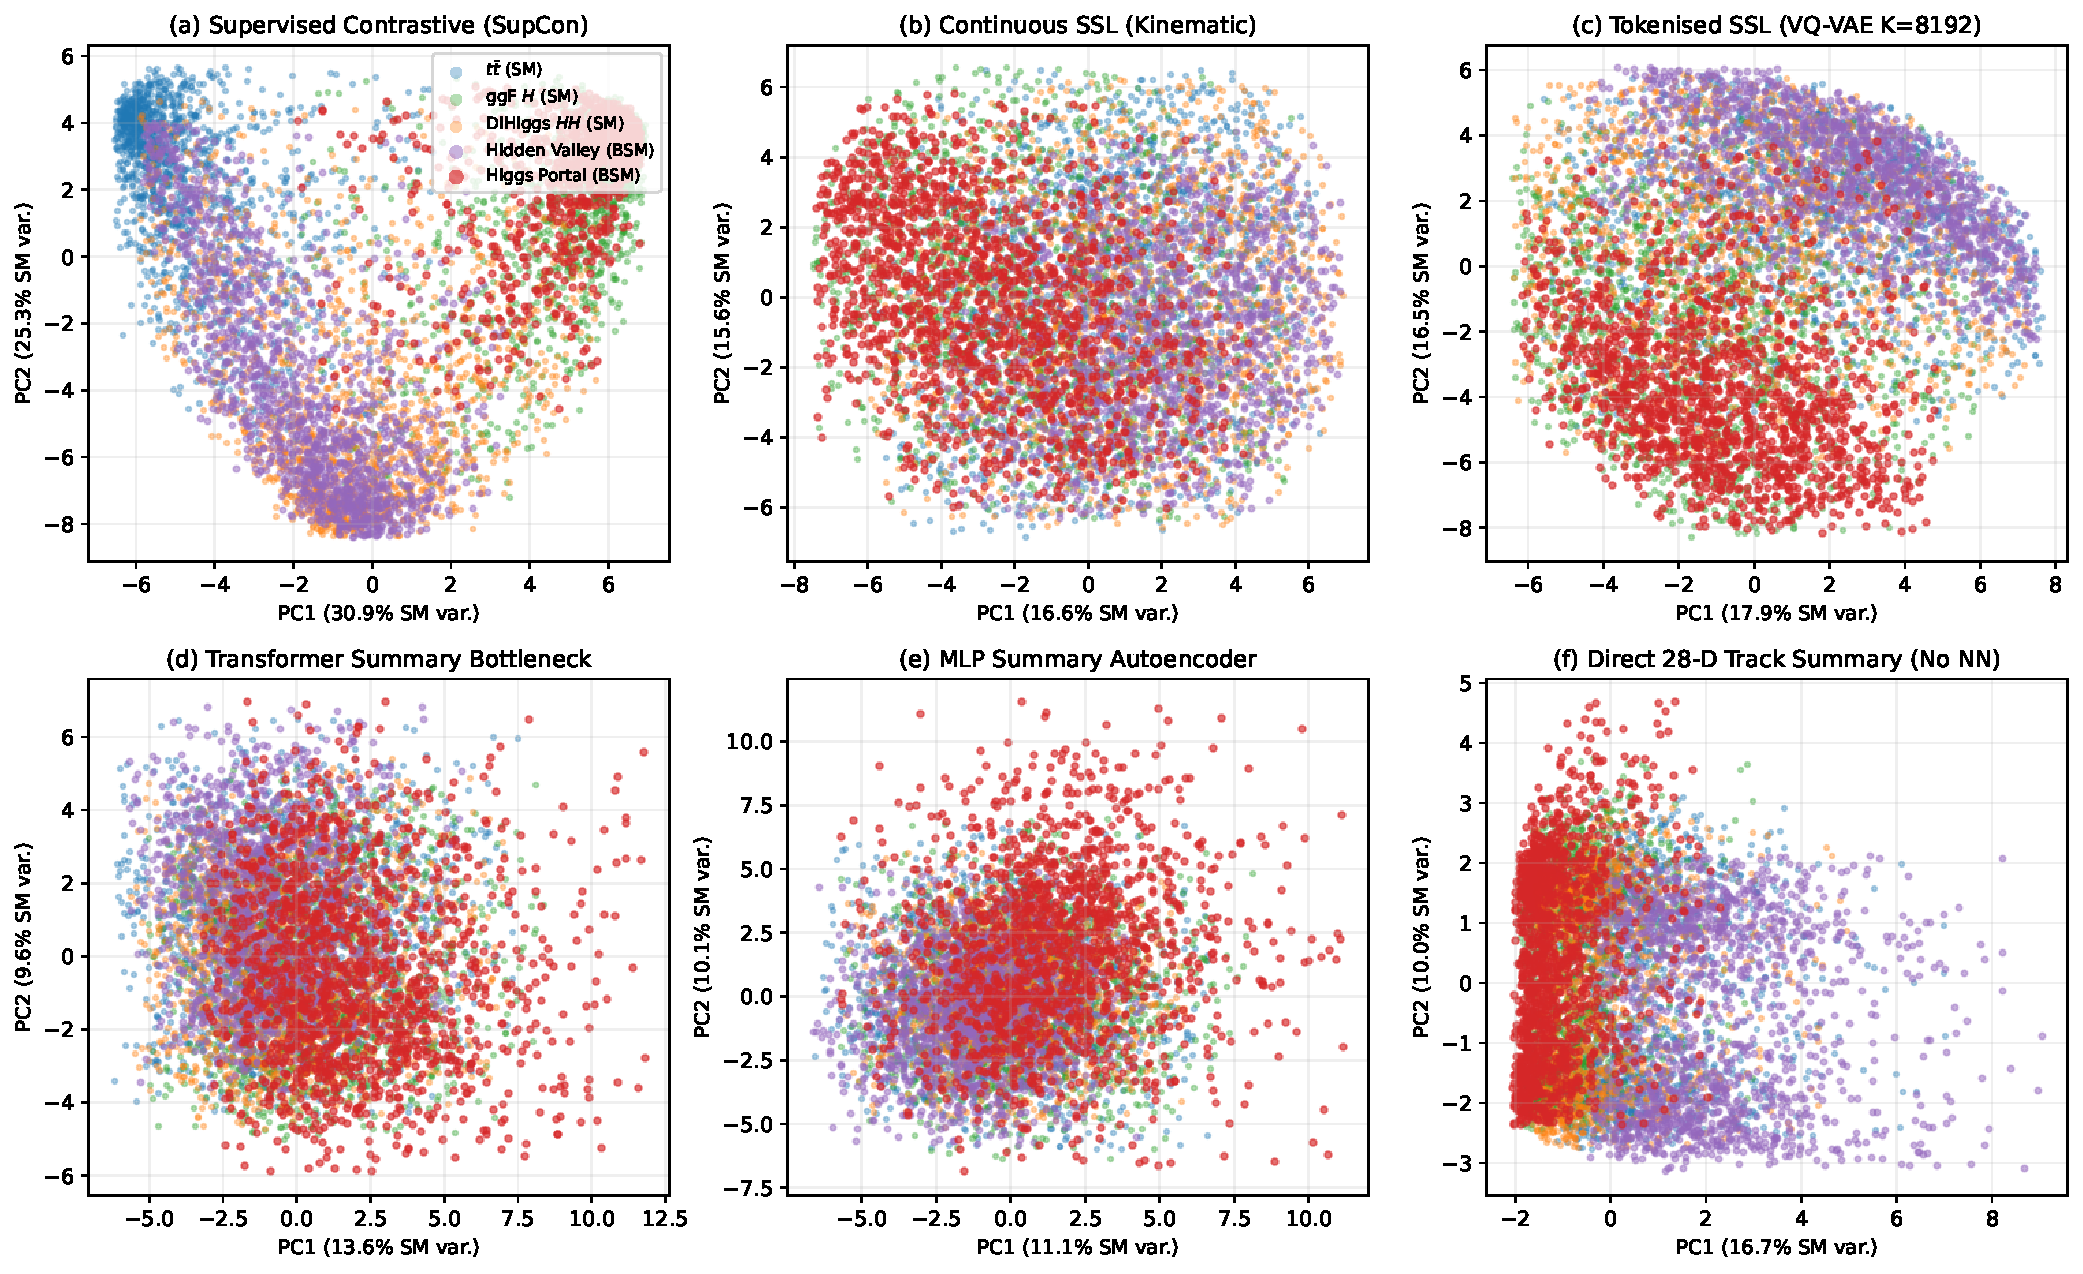
\includegraphics[width=0.97\textwidth]{fig_latent_pca_grid.pdf}
    \caption{Two-dimensional PCA projections fit to $20,000$ coordinate-standardised held-out SM embeddings across six representative models. Axis labels report the percentage of standardised SM variance captured by the leading two principal components.}
    \label{fig:latent_pca}
\end{figure}

To characterise latent geometry, we compute the Roy-Vetterli effective rank~\cite{RoyVetterli2007}, $\text{erank}_{\text{SM}} = \exp(-\sum_{k=1}^D p_k \ln p_k)$, from the normalised eigenvalues $p_k$ of the unstandardised SM covariance matrix (Table~\ref{tab:probes} in Appendix~\ref{app:probes}). Supervised SM pretraining collapses SM variance into low rank ($\text{erank}_{\text{SM}} = 2.00$ for \texttt{supervised\_e2e\_d64} and $3.50$ for \texttt{supcon\_d64}), forming three tight SM lobes in Fig.~\ref{fig:latent_pca}(a) with displaced Higgs Portal events falling in the interior region between $t\bar{t}$ and $HH$. Contrastive SSL encoders maintain intermediate effective rank ($8.30$ for \texttt{ssl\_kinematic\_d64}, $9.20$ for \texttt{ssl\_tokens\_d64}), whereas summary autoencoders span higher rank ($16.0$ to $17.2$).

\subsection{Probe Scaling and Low-Label Sample Efficiency}
\label{sec:probes}

\begin{figure}[t]
    \centering
    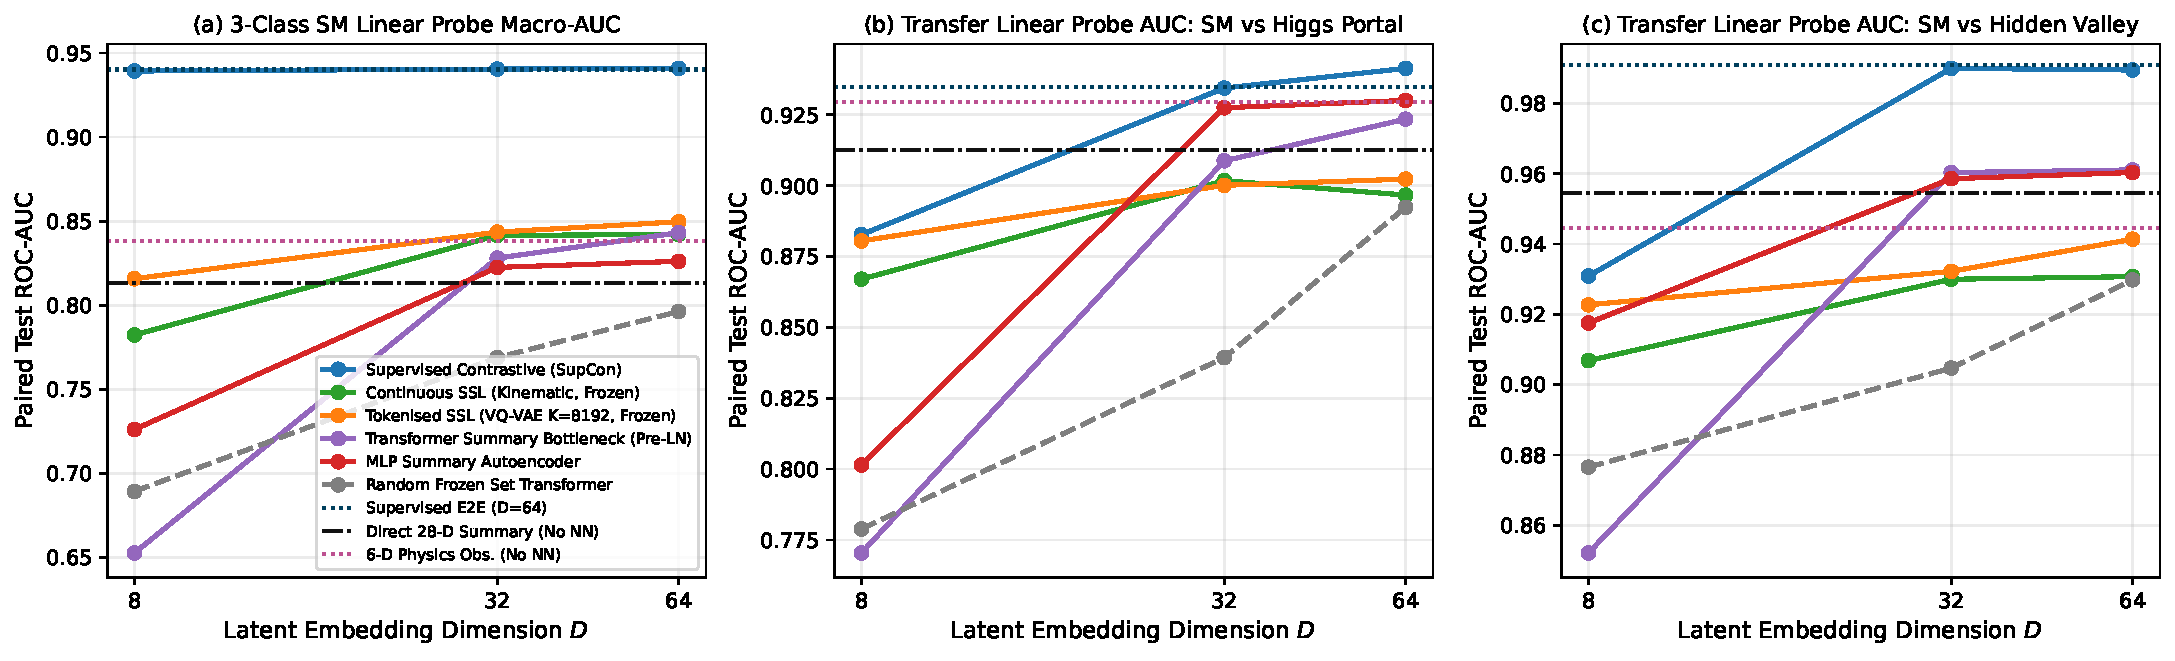
\includegraphics[width=0.97\textwidth]{fig_probe_scaling.pdf}
    \caption{Downstream linear probe ROC-AUC across bottleneck dimensions $D \in \{8, 32, 64\}$ compared with deterministic baselines (\texttt{raw\_summary\_d28} dash-dotted black, \texttt{phys\_handcrafted\_d6} dotted magenta): (a) three-class SM macro ROC-AUC, (b) binary transfer ROC-AUC on Higgs Portal, and (c) binary transfer ROC-AUC on Hidden Valley.}
    \label{fig:probe_scaling}
\end{figure}

\begin{figure}[t]
    \centering
    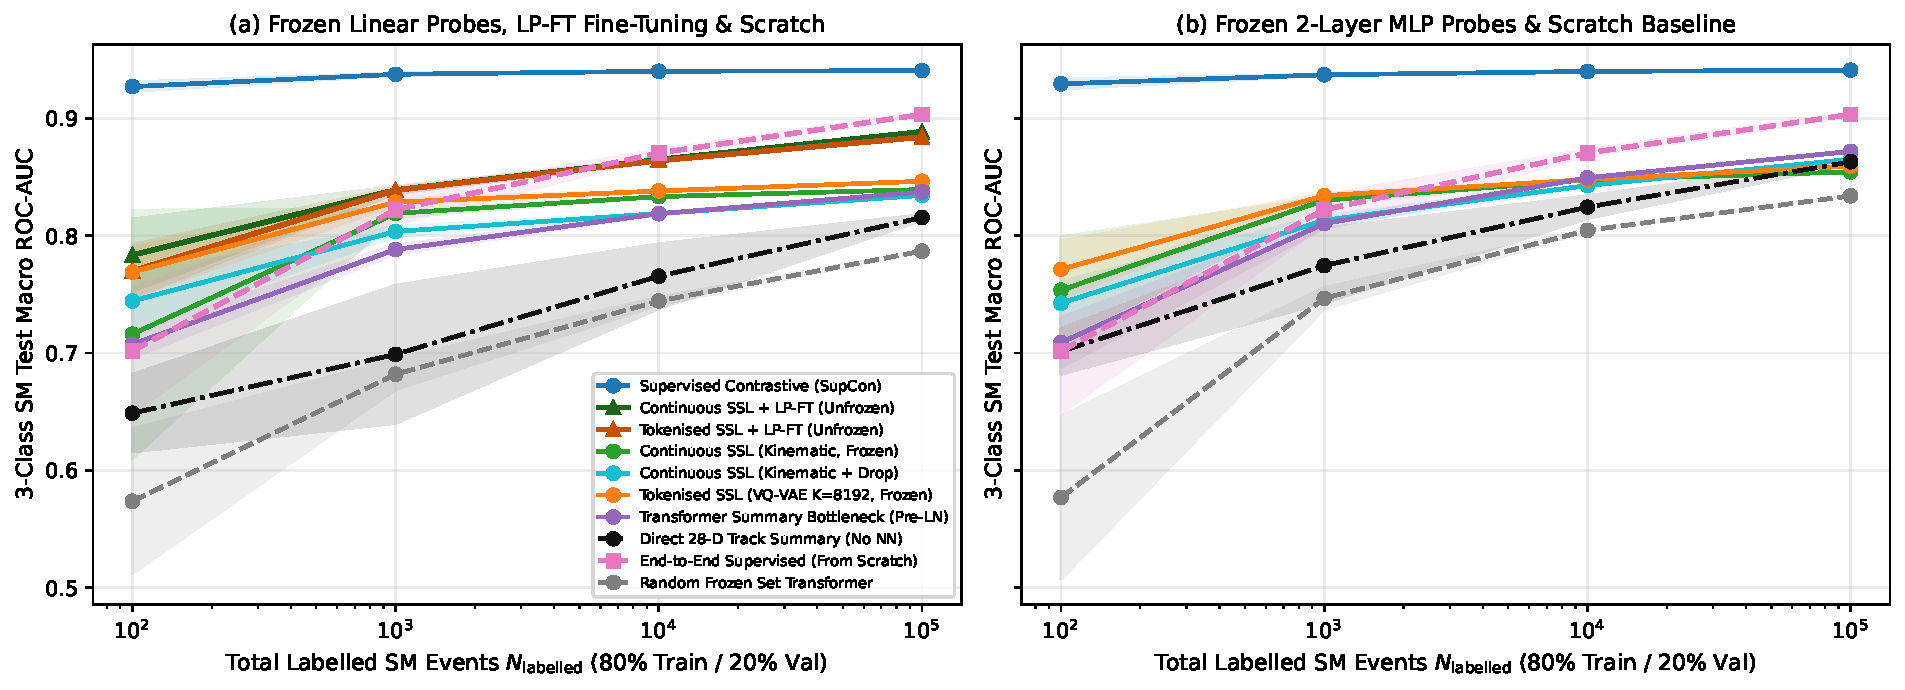
\includegraphics[width=0.97\textwidth]{fig_label_efficiency.pdf}
    \caption{Three-class SM test macro ROC-AUC across labelled SM budgets $N_{\text{labelled}} \in \{100, 10^3, 10^4, 10^5\}$ for (a) frozen linear probes and two-stage LP-FT fine-tuning, and (b) frozen two-layer MLP probes, compared with end-to-end training from random initialisation (\texttt{supervised\_scratch\_d64}) and \texttt{raw\_summary\_d28}. Points show mean $\pm 1\sigma$ across five paired draws.}
    \label{fig:label_eff}
\end{figure}

Linear probe scaling across $D \in \{8, 32, 64\}$ is shown in Fig.~\ref{fig:probe_scaling} (full 27-model results in Table~\ref{tab:probes} and three-seed reproducibility in Table~\ref{tab:seed_lpft}, Appendix~\ref{app:probes}):
\begin{enumerate}
    \item \emph{Continuous and discrete SSL scaling.} Three-class SM linear accuracy rises monotonically from $0.6031$ ($D=8$) to $0.6800$ ($D=64$; three-seed mean $0.6790 \pm 0.0019$) for \texttt{ssl\_kinematic}, and from $0.6439$ ($D=8$) to $0.6893$ ($D=64$; three-seed mean $0.6858 \pm 0.0079$) for \texttt{ssl\_tokens}. Adding $10\%$ random track dropping (\texttt{ssl\_kinematic\_drop\_d64}) lifts two-layer MLP SM-3 accuracy to $0.7230$. Pre- and post-quantisation VQ-VAE poolings (\texttt{vqvae\_code\_d8} vs.\ \texttt{vqvae\_quant\_d8}) agree within $0.0023$ on every metric, confirming lossless $K=8192$ discretisation for downstream probing.
    \item \emph{Comparison against physics baselines.} Without learned parameters, \texttt{raw\_summary\_d28} reaches $0.6413$ linear ($0.7117$ MLP) SM-3 accuracy and \texttt{phys\_handcrafted\_d6} reaches $0.6747$ linear accuracy with $0.9296$ Higgs Portal transfer AUC. Full-set contrastive Transformers surpass \texttt{raw\_summary\_d28} by $4$ to $5$ percentage points on linear SM classification, while \texttt{vqvae\_encoder\_d128} attains the highest unsupervised transfer AUCs ($0.9549$ on Higgs Portal, $0.9774$ on Hidden Valley).
    \item \emph{Low-label efficiency and LP-FT fine-tuning (Fig.~\ref{fig:label_eff}).} At $N_{\text{labelled}} = 100$, training the Set Transformer from scratch (\texttt{supervised\_scratch\_d64}) yields $52.3\% \pm 7.2\%$ accuracy, whereas frozen probing on \texttt{ssl\_tokens\_d64} reaches $58.5\% \pm 2.9\%$ and LP-FT fine-tuning of \texttt{ssl\_kinematic\_d64} reaches $61.2\% \pm 3.4\%$. At $N_{\text{labelled}} = 1,000$, LP-FT reaches $67.8\% \pm 0.5\%$ (\texttt{ssl\_kinematic\_ft\_d64}) versus $65.2\% \pm 2.8\%$ from scratch, cutting seed-to-seed variance sixfold, while unfreezing the backbone eliminates the frozen-probe ceiling at $10^4$ to $10^5$ labels ($74.5\%$).
\end{enumerate}

\section{Model-Independent Anomaly Detection with Kernel NPLM}
\label{sec:nplm}

\subsection{Kernel Log-Likelihood Ratio Formulation and Calibration}
\label{sec:nplm_calibration}

Kernel NPLM~\cite{NPLM2019,NPLM2021,KernelNPLM2022} tests whether an experimental dataset $\mathcal{D}$ of size $N_D$ deviates from a Standard Model reference sample $\mathcal{R}$ of size $N_R$ without specifying an alternative signal hypothesis. Standardising embeddings per coordinate on $\mathcal{R}$ only and drawing $M$ Nystr\"om centres $\{c_1, \dots, c_M\} \subset \mathcal{R}$, each embedding $\mathbf{x} \in \mathbb{R}^D$ is mapped via a Gaussian kernel of width $\sigma$ to $\boldsymbol{\phi}(\mathbf{x}) = [K(\mathbf{x}, c_1), \dots, K(\mathbf{x}, c_M)]^\top \in \mathbb{R}^M$, where $K(\mathbf{x}, c_i) = \exp(-\|\mathbf{x} - c_i\|_2^2 / 2\sigma^2)$. Approximating the log-intensity ratio $\log[N_D p_D(\mathbf{x}) / N_B p_B(\mathbf{x})]$ by $f_{\mathbf{w}}(\mathbf{x}) = \boldsymbol{\phi}(\mathbf{x})^\top \mathbf{w}$, the weight vector $\mathbf{w} \in \mathbb{R}^M$ minimises the $K_{MM}$-regularised weighted logistic loss ($y=0$ for $\mathbf{x}\in\mathcal{R}$, $y=1$ for $\mathbf{x}\in\mathcal{D}$, with $a_0 = 1$ and $a_1 = N_R / N_B$ matching Eq.~(12) of Ref.~\cite{KernelNPLM2022}):
\begin{equation}
    \mathcal{J}(\mathbf{w}) = \sum_{\mathbf{x} \in \mathcal{R}} \log\big(1 + e^{f_{\mathbf{w}}(\mathbf{x})}\big) + \frac{N_R}{N_B}\sum_{\mathbf{y} \in \mathcal{D}} \log\big(1 + e^{-f_{\mathbf{w}}(\mathbf{y})}\big) + \frac{\lambda}{2}\,\mathbf{w}^\top K_{MM}\mathbf{w} ,
\end{equation}
yielding the extended log-likelihood ratio test statistic
\begin{equation}
    t_{\mathbf{w}} = 2\left[\frac{N_B}{N_R}\sum_{\mathbf{x} \in \mathcal{R}}\big(1 - e^{f_{\mathbf{w}}(\mathbf{x})}\big) + \sum_{\mathbf{y} \in \mathcal{D}} f_{\mathbf{w}}(\mathbf{y})\right] .
\end{equation}

Because additive injection ($N_D = N_B + N_S$) introduces a representation-independent Poisson rate term $t_{\text{rate}} \approx N_S^2 / N_B$ even for a constant model $f_0 = \log(N_D / N_B)$ (verified in Appendix~\ref{app:nplm} and Fig.~\ref{fig:nplm_cal}), all primary benchmarks use fixed-size shape-only mixtures ($N_D = N_B = 100,000$, replacing $N_S$ background events with signal events so $t_{\text{rate}} \equiv 0$). In our primary $10,000$-null benchmark ($N_R = 500,000$, $250,000$-event held-out SM pool, $M = 316$, $q = 0.90$ pairwise distance quantile, $\lambda = 10^{-6}$), we solve each toy to machine precision in $\sim 30\text{ ms}$ via damped GPU \texttt{float64} Newton-Raphson steps (Appendix~\ref{app:nplm}), set exact order-statistic thresholds $t_{1-\alpha}$~\cite{PhipsonSmyth2010} on $5,000$ calibration nulls, and verify out-of-sample false-positive control on $5,000$ independent validation nulls with Clopper-Pearson intervals~\cite{ClopperPearson1934}.

\subsection{Sensitivity Across Displaced and Dark-Shower Topologies}
\label{sec:nplm_results}

\begin{table}[t!]
\centering
\caption{Conditional $10,000$-null shape-only Kernel NPLM benchmark across 16 representative models ($N_R = 500\text{k}$, $N_D = N_B = 100\text{k}$; $5,000$ calibration nulls, $5,000$ validation nulls, $200$ paired signal toys per point). Columns report out-of-sample validation false-positive rates, empirical power at $\alpha = 10^{-3}$ with $95\%$ Clopper-Pearson intervals, and standardised median shift $\text{SNR} = (t_{\text{med}}-\mu_{\text{null}})/\sigma_{\text{null}}$ with $[q_{16}, q_{84}]$ intervals.}
\label{tab:nplm_highstats}
\resizebox{\linewidth}{!}{%
\begin{tabular}{llcc|ccc|ccc}
\toprule
& & \multicolumn{2}{c|}{\textbf{Validation FPR ($5\text{k}$)}} & \multicolumn{3}{c|}{\textbf{Higgs Portal (Displaced LLP)}} & \multicolumn{3}{c}{\textbf{Hidden Valley (Dark Shower)}} \\
\textbf{Model} & $D$ & $\alpha=10^{-2}$ & $\alpha=10^{-3}$ & $\textbf{Pow}_{10^{-3}}\text{ (0.5\%)}$ & $\textbf{Pow}_{10^{-3}}\text{ (1.0\%) [95\% CI]}$ & $\textbf{SNR}_{1\%}\text{ }[q_{16},q_{84}]$ & $\textbf{Pow}_{10^{-3}}\text{ (0.5\%)}$ & $\textbf{Pow}_{10^{-3}}\text{ (1.0\%) [95\% CI]}$ & $\textbf{SNR}_{1\%}\text{ }[q_{16},q_{84}]$ \\
\midrule
\texttt{supcon\_d64} & 64 & 0.0090 & 0.0016 & 0.035 & 0.695 [0.626, 0.758] & 3.57 [2.49, 4.82] & \textbf{1.000} & \textbf{1.000 [0.982, 1.000]} & \textbf{34.97 [32.87, 37.27]} \\
\texttt{supervised\_e2e\_d64} & 64 & 0.0118 & 0.0016 & 0.000 & 0.185 [0.134, 0.246] & 2.38 [1.26, 3.35] & 0.550 & \textbf{1.000 [0.982, 1.000]} & 14.89 [13.48, 16.37] \\
\midrule
\texttt{ssl\_kinematic\_d32} & 32 & 0.0094 & 0.0000 & 0.005 & 0.615 [0.544, 0.683] & 4.20 [2.68, 5.17] & 0.000 & 0.595 [0.523, 0.664] & 4.17 [2.97, 5.20] \\
\texttt{ssl\_kinematic\_d64} & 64 & 0.0114 & 0.0004 & 0.005 & 0.485 [0.414, 0.557] & 3.48 [2.12, 4.49] & 0.010 & 0.770 [0.705, 0.826] & 4.14 [3.26, 5.26] \\
\texttt{ssl\_tokens\_d8} & 8 & 0.0078 & 0.0014 & 0.045 & 0.960 [0.923, 0.983] & 5.58 [4.37, 7.03] & 0.085 & 0.995 [0.972, 1.000] & 6.83 [5.60, 8.59] \\
\texttt{ssl\_tokens\_d32} & 32 & 0.0082 & 0.0010 & 0.025 & 0.790 [0.727, 0.844] & 4.19 [3.04, 5.46] & 0.015 & 0.925 [0.879, 0.957] & 4.84 [3.84, 6.22] \\
\texttt{ssl\_tokens\_d64} & 64 & 0.0088 & 0.0004 & 0.030 & 0.720 [0.652, 0.781] & 4.04 [2.95, 5.26] & 0.025 & 0.870 [0.815, 0.913] & 4.86 [3.60, 6.19] \\
\midrule
\texttt{ae\_transformer\_d32} & 32 & 0.0078 & 0.0010 & 0.090 & \textbf{1.000 [0.982, 1.000]} & 7.83 [6.38, 9.38] & 0.080 & \textbf{1.000 [0.982, 1.000]} & 6.56 [5.13, 7.80] \\
\texttt{ae\_mlp\_d32} & 32 & 0.0106 & 0.0014 & 0.155 & \textbf{1.000 [0.982, 1.000]} & 8.19 [6.64, 9.82] & 0.030 & 0.915 [0.867, 0.950] & 4.74 [3.65, 6.04] \\
\texttt{vqvae\_code\_d8} (pure $\mathbf{z}_e$) & 8 & 0.0104 & 0.0020 & 0.850 & \textbf{1.000 [0.982, 1.000]} & 17.34 [14.93, 19.72] & 0.000 & 0.070 [0.039, 0.115] & 1.65 [0.68, 2.63] \\
\texttt{vqvae\_quant\_d8} (pure $\mathbf{z}_q$) & 8 & 0.0082 & 0.0010 & 0.830 & \textbf{1.000 [0.982, 1.000]} & 17.11 [14.90, 19.46] & 0.000 & 0.045 [0.021, 0.084] & 1.57 [0.48, 2.53] \\
\texttt{random\_init\_d64} & 64 & 0.0092 & 0.0006 & 0.005 & 0.550 [0.478, 0.620] & 3.54 [2.33, 4.85] & 0.030 & 0.965 [0.929, 0.986] & 5.07 [3.99, 6.41] \\
\midrule
\texttt{raw\_summary\_d28} (no NN) & 28 & 0.0082 & 0.0016 & 0.250 & \textbf{1.000 [0.982, 1.000]} & 8.67 [6.97, 10.28] & 0.060 & 0.975 [0.943, 0.992] & 5.30 [4.11, 6.57] \\
\texttt{pca\_summary\_d8} (no NN) & 8 & 0.0102 & 0.0020 & 0.305 & \textbf{1.000 [0.982, 1.000]} & 9.81 [8.15, 11.86] & 0.010 & 0.560 [0.488, 0.630] & 3.44 [2.39, 4.49] \\
\texttt{phys\_handcrafted\_d6} (no NN) & 6 & 0.0132 & 0.0010 & \textbf{1.000} & \textbf{1.000 [0.982, 1.000]} & \textbf{28.02 [24.70, 31.61]} & 0.095 & \textbf{1.000 [0.982, 1.000]} & 8.80 [6.78, 10.40] \\
\texttt{mult\_only\_d1} (no NN) & 1 & 0.0102 & 0.0004 & 0.015 & 0.480 [0.409, 0.552] & 4.64 [2.86, 7.17] & 0.000 & 0.000 [0.000, 0.018] & 0.44 [-0.64, 1.69] \\
\bottomrule
\end{tabular}%
}
\end{table}

\begin{figure}[t]
    \centering
    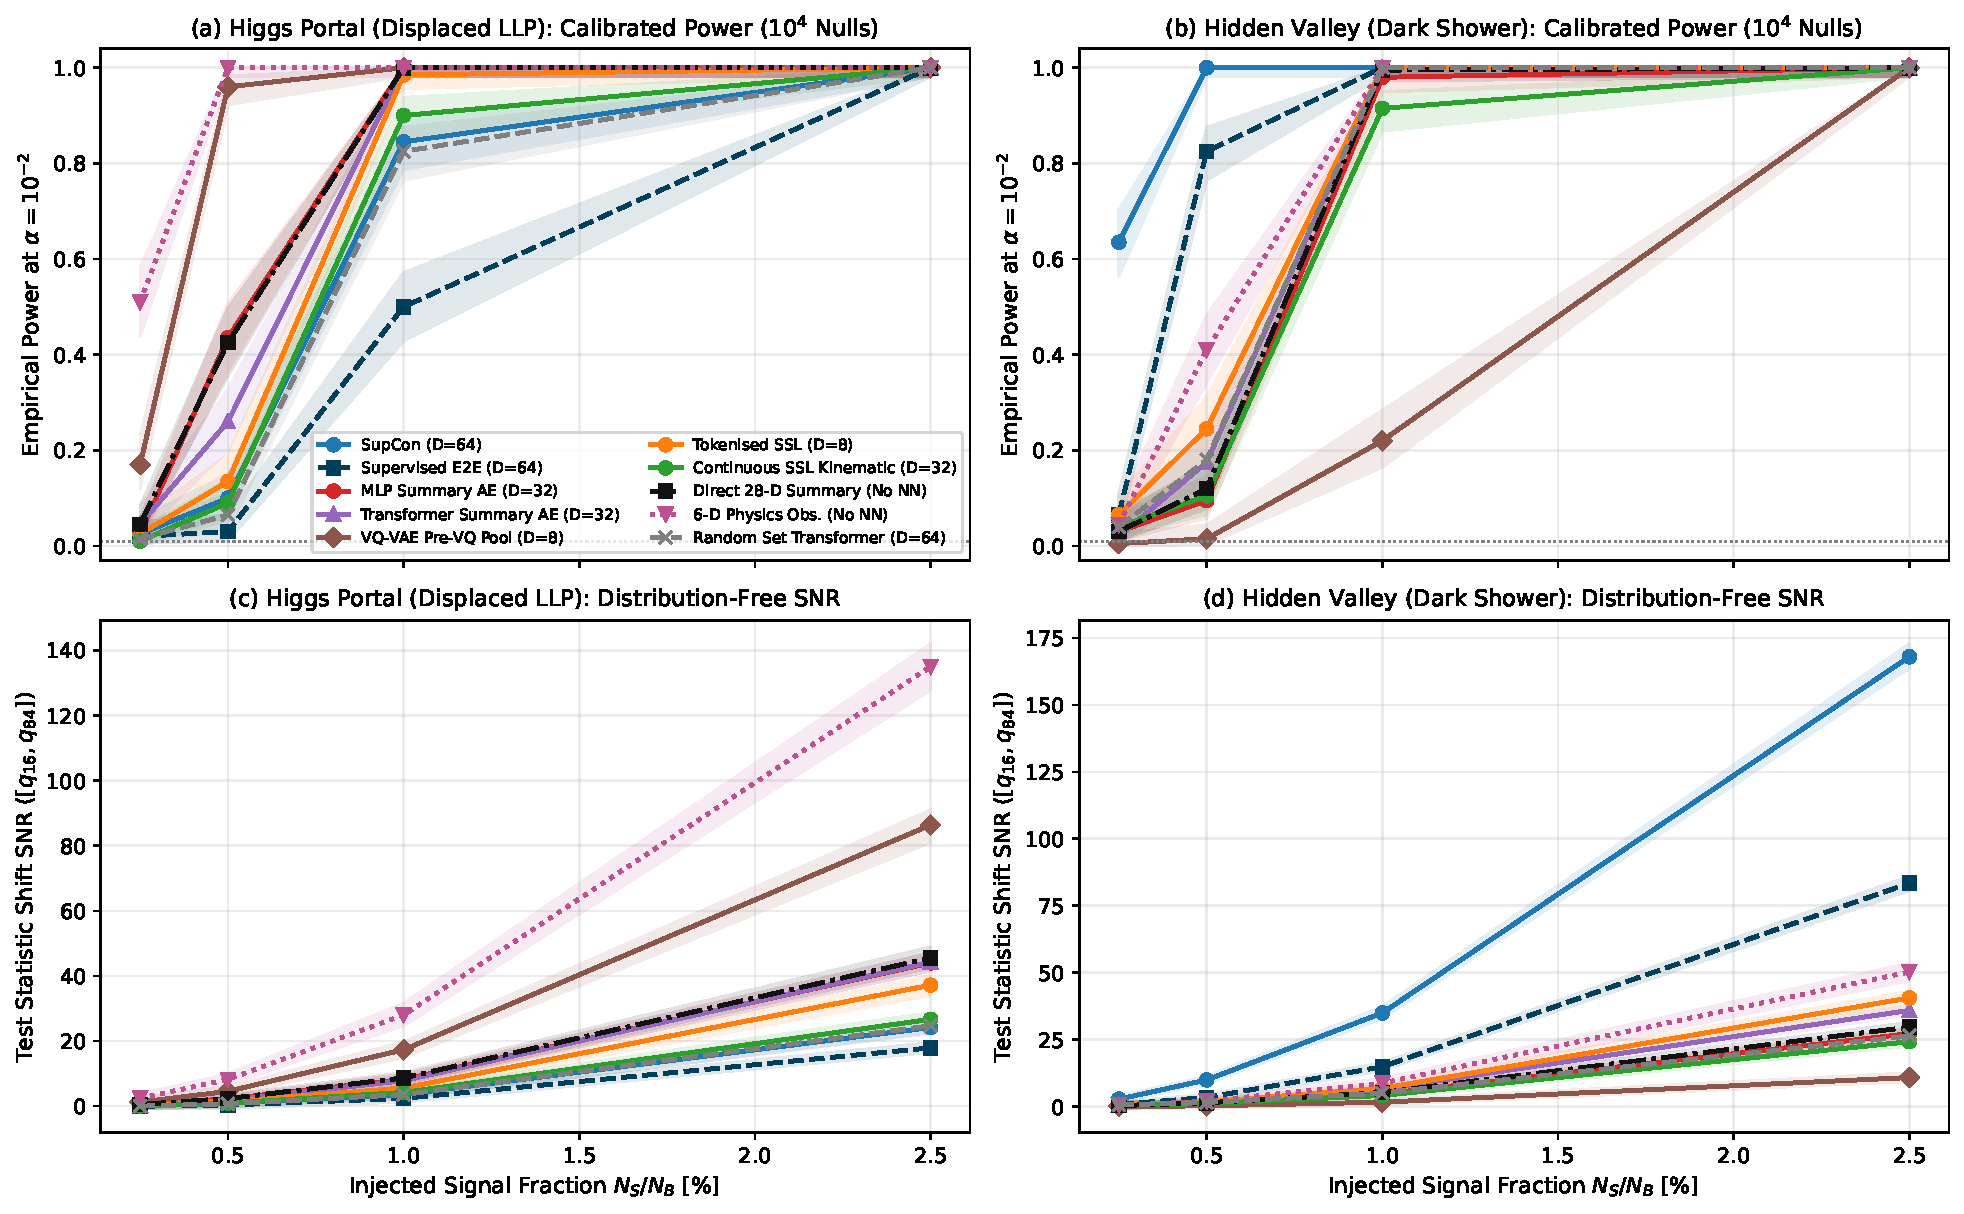
\includegraphics[width=0.97\textwidth]{fig_nplm_significance_curves.pdf}
    \caption{Conditional $10,000$-null shape-only Kernel NPLM detection curves across signal fractions from $0.25\%$ to $2.5\%$ ($200$ signal toys per point): (a, b) empirical power at $\alpha = 10^{-2}$ with $95\%$ Clopper-Pearson bands, and (c, d) standardised median shift $\text{SNR}$ with $[q_{16}, q_{84}]$ intervals on Higgs Portal (left) and Hidden Valley (right).}
    \label{fig:nplm_curves}
\end{figure}

Results from the $10,000$-null benchmark are shown in Table~\ref{tab:nplm_highstats} and Fig.~\ref{fig:nplm_curves} (full 27-model sweep in Table~\ref{tab:nplm}, Appendix~\ref{app:nplm}). Model rankings reverse between the two BSM channels and differ from the supervised probe rankings. On Hidden Valley dark showers, SM-supervised contrastive embeddings lead ($\text{SNR}_{1\%} = 34.97$ for \texttt{supcon\_d64}, achieving unit power at $\alpha = 10^{-3}$ down to $0.5\%$ injection). On displaced Higgs Portal decays at $1.0\%$ injection, however, \texttt{supervised\_e2e\_d64} drops to $\text{Pow}_{10^{-3}} = 0.185$ ($\text{SNR}_{1\%} = 2.38$) and \texttt{supcon\_d64} drops to $\text{SNR}_{1\%} = 3.57$. Instead, the compact $D=8$ VQ-VAE poolings lead all neural models on Higgs Portal ($\text{SNR}_{1\%} = 17.34$ and $17.11$, with $\text{Pow}_{10^{-3}} = 0.830$ to $0.850$ at $0.5\%$ injection), followed by the 28-D summary autoencoders ($\text{SNR}_{1\%} = 7.83$ to $8.19$) and balanced tokenised SSL (\texttt{ssl\_tokens\_d8}, $\text{Pow}_{10^{-3}} = 0.960$ on Higgs Portal and $0.995$ on Hidden Valley). Across all 27 representations, the deterministic six-observable baseline \texttt{phys\_handcrafted\_d6} attains the highest Higgs Portal sensitivity ($\text{SNR}_{1\%} = 28.02$) alongside strong Hidden Valley sensitivity ($\text{SNR}_{1\%} = 8.80$).

\subsection{Tracking Efficiency, Masking, and Kernel-Geometry Controls}
\label{sec:physics_controls}

\begin{figure}[t]
    \centering
    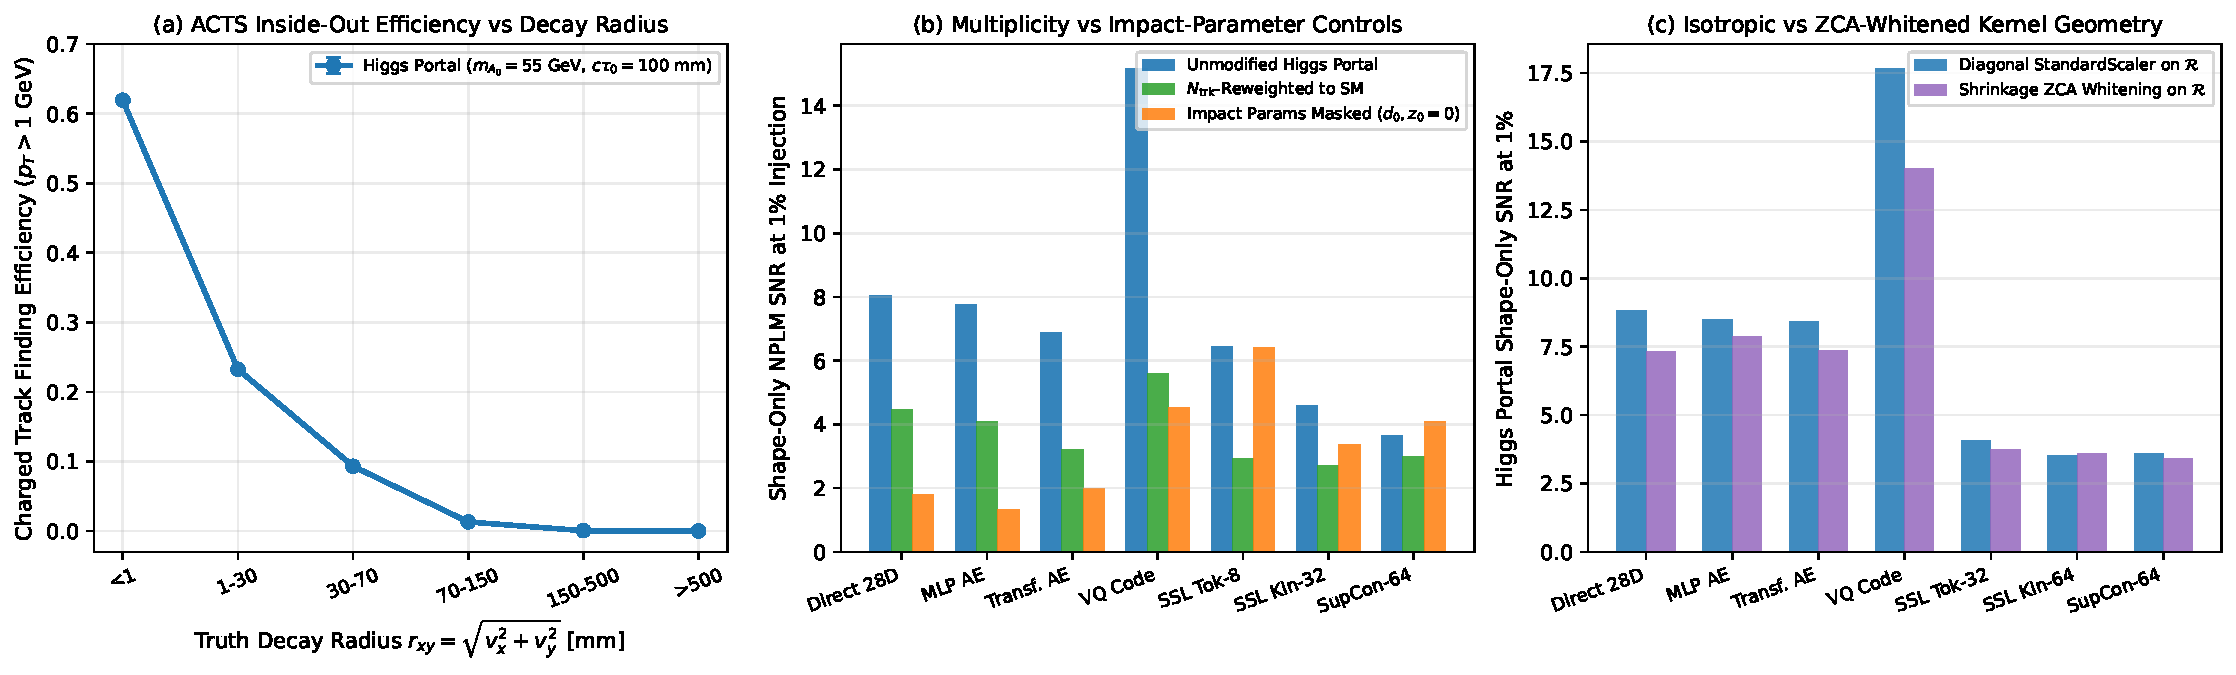
\includegraphics[width=0.97\textwidth]{fig_physics_controls.pdf}
    \caption{Detector tracking, masking, and kernel-geometry controls on Higgs Portal decays: (a) truth-matched \textsc{ACTS} inside-out track-finding efficiency ($p_T > 1\text{ GeV}$, $|\eta| < 3.0$) versus transverse decay radius $r_{xy}$; (b) $1\%$ shape-only NPLM $\text{SNR}$ comparing unmodified displaced events, SM track-multiplicity-reweighted events, and $(d_0, z_0)=0$ impact-parameter-masked events; and (c) diagonal \texttt{StandardScaler} versus shrinkage ZCA covariance whitening on $\mathcal{R}$.}
    \label{fig:physics_controls}
\end{figure}

Physical and geometric controls for this ranking reversal are shown in Fig.~\ref{fig:physics_controls} and Table~\ref{tab:roc_tail} (Appendix~\ref{app:nplm}):
\begin{enumerate}
    \item \emph{Inside-out seeding drop-off and impact-parameter masking.} Matching truth charged particles ($p_T > 1\text{ GeV}$, $|\eta| < 3.0$) via hit barcodes shows that \textsc{ACTS} inside-out efficiency falls from $61.9\%$ below $r_{xy} = 1\text{ mm}$ to $9.3\%$ between $30$ and $70\text{ mm}$ and $0.03\%$ beyond $150\text{ mm}$ (Fig.~\ref{fig:physics_controls}a). Reweighting signal toys to match the SM track-multiplicity histogram eliminates multiplicity-only sensitivity ($\text{SNR}_{1\%}: 5.31 \to 0.06$) while retaining $\text{SNR}_{1\%} = 16.82$ for \texttt{phys\_handcrafted\_d6} and $5.69$ for \texttt{vqvae\_quant\_d8} (Fig.~\ref{fig:physics_controls}b). Conversely, zeroing $d_0 = z_0 = 0$ prior to scaling collapses multiplicity-matched $\text{SNR}_{1\%}$ in \texttt{raw\_summary\_d28} ($4.46 \to 0.34$) and \texttt{vqvae\_quant\_d8} ($5.69 \to 1.10$), confirming genuine reliance on displaced perigee tails.
    \item \emph{ROC-tail crossover and coordinate dilution.} Although \texttt{supcon\_d64} achieves higher integrated binary ROC-AUC on Higgs Portal ($0.9414$) than \texttt{vqvae\_quant\_d8} ($0.9118$), evaluating binary probes against $702,000$ held-out SM events shows that their ROC curves cross in the high-purity tail (Table~\ref{tab:roc_tail}): at $\text{FPR} = 10^{-3}$ and $10^{-4}$, \texttt{supcon\_d64} drops to $2.7\%$ and $0.34\%$ recall because displaced events lie between SM class lobes (Fig.~\ref{fig:latent_pca}a), whereas \texttt{vqvae\_quant\_d8} ($11.5\%$, $3.13\%$) and \texttt{ae\_transformer\_d32} ($12.8\%$, $3.25\%$) retain four- to tenfold higher extreme-tail efficiency. Isotropic Euclidean kernels also weight all $D$ standardised coordinates equally (even after shrinkage ZCA whitening, Fig.~\ref{fig:physics_controls}c), rewarding compact $D=6$ to $8$ representations that concentrate displaced-tail information without diluting $\|\mathbf{z} - c_i\|_2^2$ across dozens of background-dominated directions.
\end{enumerate}

\begin{dmbox}[New Subsection for Review: Comparison to LHC Exclusion Limits and Sample-Size Scaling]
\subsection{Interpreting Sensitivity Against LHC Exclusion Limits and Sample-Size Scaling}
\label{sec:exclusion_limits}

To situate our sub-percent injection benchmarks physically, we relate the injected signal fraction $f = N_S / N_D$ to $14\text{ TeV}$ production cross sections and existing LHC exclusion bounds, while highlighting two structural differences between a benchmark dataset mixture and an inclusive collider search. Summing the three simulated SM channels at $\sqrt{s} = 14\text{ TeV}$ gives $\sigma(t\bar{t}) \approx 955\text{ pb}$ at NNLO+NNLL~\cite{Czakon2013}, $\sigma(\text{ggF } H) \approx 54.7\text{ pb}$~\cite{LHCHXSWG4}, and $\sigma(HH) \approx 0.036\text{ pb}$~\cite{LHCHXSWG4}, for a combined three-process cross section $\sigma_{\text{3SM}} \approx 1,010\text{ pb}$.

In the Higgs Portal model ($H \to A_0 A_0 \to 4b$ at $m_{A_0} = 55\text{ GeV}$, $c\tau_0 = 100\text{ mm}$), the exotic branching fraction $\text{BR}(H \to A_0 A_0)$ is controlled by the independent portal coupling $\lambda_{Haa}$ rather than fixed by $(m_{A_0}, c\tau_0)$. Combined Run-2 Higgs coupling fits constrain undetermined or exotic Higgs decays to $\text{BR}_{\text{exotic}} \le 12\%$ at $95\%\text{ CL}$~\cite{ATLASHiggsNature2022}, corresponding to $\sigma_{\text{HP}} \le 6.6\text{ pb}$ or $\sigma_{\text{HP}} / \sigma_{\text{3SM}} \approx 0.65\%$. Dedicated Run-2 ($140\text{ fb}^{-1}$) inner-detector displaced-vertex searches by ATLAS~\cite{ATLASDV2024} tighten this bound at $(55\text{ GeV}, 100\text{ mm})$ by an order of magnitude to $\text{BR}(H \to A_0 A_0 \to 4b) \lesssim 1.3\%$ ($\sigma_{\text{HP}} \lesssim 0.71\text{ pb}$, or $\sigma_{\text{HP}} / \sigma_{\text{3SM}} \approx 0.07\%$). Both experimental limits are upper bounds compatible with zero signal; crucially, $\text{BR} \approx 1.3\%$ in Ref.~\cite{ATLASDV2024} is a fraction of $\text{ggF } H$ events alone rather than $1.3\%$ of $N_D$. In addition, our evaluation sample mixes $(t\bar{t}, \text{ggF } H, HH)$ in unweighted $1{:}1{:}1$ proportions while omitting multijet QCD backgrounds, and Kernel NPLM operates on inclusive track embeddings without reconstructing secondary vertices or specifying a signal template. For the Hidden Valley benchmark ($\Lambda_v = 40\text{ GeV}$), \textsc{Pythia}~8.3 gives a leading-order cross section $\sigma_{\text{HV}} \approx 4.41\text{ pb}$ ($\sigma_{\text{HV}} / \sigma_{\text{3SM}} \approx 0.44\%$), a picobarn-scale dark-shower rate probed by dedicated LHC emerging-jet searches~\cite{CMSEmergingJets2024}.

Sub-percent detection power and event-count scaling under full joint $(\mathcal{R}, \mathcal{D})$ resampling ($M = 1,000$ centres) are shown in Fig.~\ref{fig:exclusion_scaling}. Scaling $N_D$ from $100\text{k}$ to $250\text{k}$ ($N_R = 500\text{k}$) and $480\text{k}$ ($N_R = 1\text{M}$) substantially improves sensitivity at fixed branching fractions:
\begin{itemize}
    \item At $f = 0.50\%$ (below the inclusive $\text{BR}_{\text{exotic}} \le 12\%$ cross-section ratio of $0.65\%$ and near the Hidden Valley LO ratio of $0.44\%$), calibrated $\alpha = 10^{-2}$ power on Higgs Portal rises from $6\%$ ($100\text{k}$) to $84\%$ ($250\text{k}$) for \texttt{ae\_transformer\_d32} ($100\%$ at $480\text{k}$), from $64\%$ to $100\%$ for \texttt{vqvae\_quant\_d8}, and from $26\%$ to $62\%$ for \texttt{ssl\_tokens\_d8}.
    \item At $f = 0.25\%$ (Fig.~\ref{fig:exclusion_scaling}c,d), median shift $\text{SNR}$ climbs monotonically out of the $\pm 1\sigma$ null band with sample size: on Hidden Valley, \texttt{SupCon} jumps from $20\%$ to $26\%$ power at $100\text{k}$ up to $84\%$ to $100\%$ at $250\text{k}$ and $480\text{k}$ (retaining $64\%$ power even at $f = 0.15\%$ for $N_D = 480\text{k}$); on Higgs Portal, \texttt{phys\_handcrafted\_d6} rises from $28\%$ ($100\text{k}$) to $68\%$ ($250\text{k}$) and \texttt{vqvae\_quant\_d8} rises from $2\%$ to $30\%$.
\end{itemize}
At the dedicated displaced-vertex upper limit ($\sigma_{\text{HP}} / \sigma_{\text{3SM}} \approx 0.07\%$), all representations remain consistent with the null at $N_D \le 480\text{k}$: signal-agnostic full-event testing without vertex reconstruction exhibits an $\mathcal{O}(3\text{ to }7\times)$ sensitivity gap in three-process signal fraction relative to dedicated Run-2 displaced-vertex reconstruction (and a wider gap once realistic multijet trigger streams are included). Because joint $(\mathcal{R}, \mathcal{D})$ variance acquires a finite-reference penalty when $N_D / N_R \to 0.5$, closing this gap further scales as $f_{\text{min}} \propto N_D^{-1/2}$ provided reference statistics scale commensurately ($N_R \gg N_D$).
\end{dmbox}

\begin{figure}[t]
\dmfloat{%
    \centering
    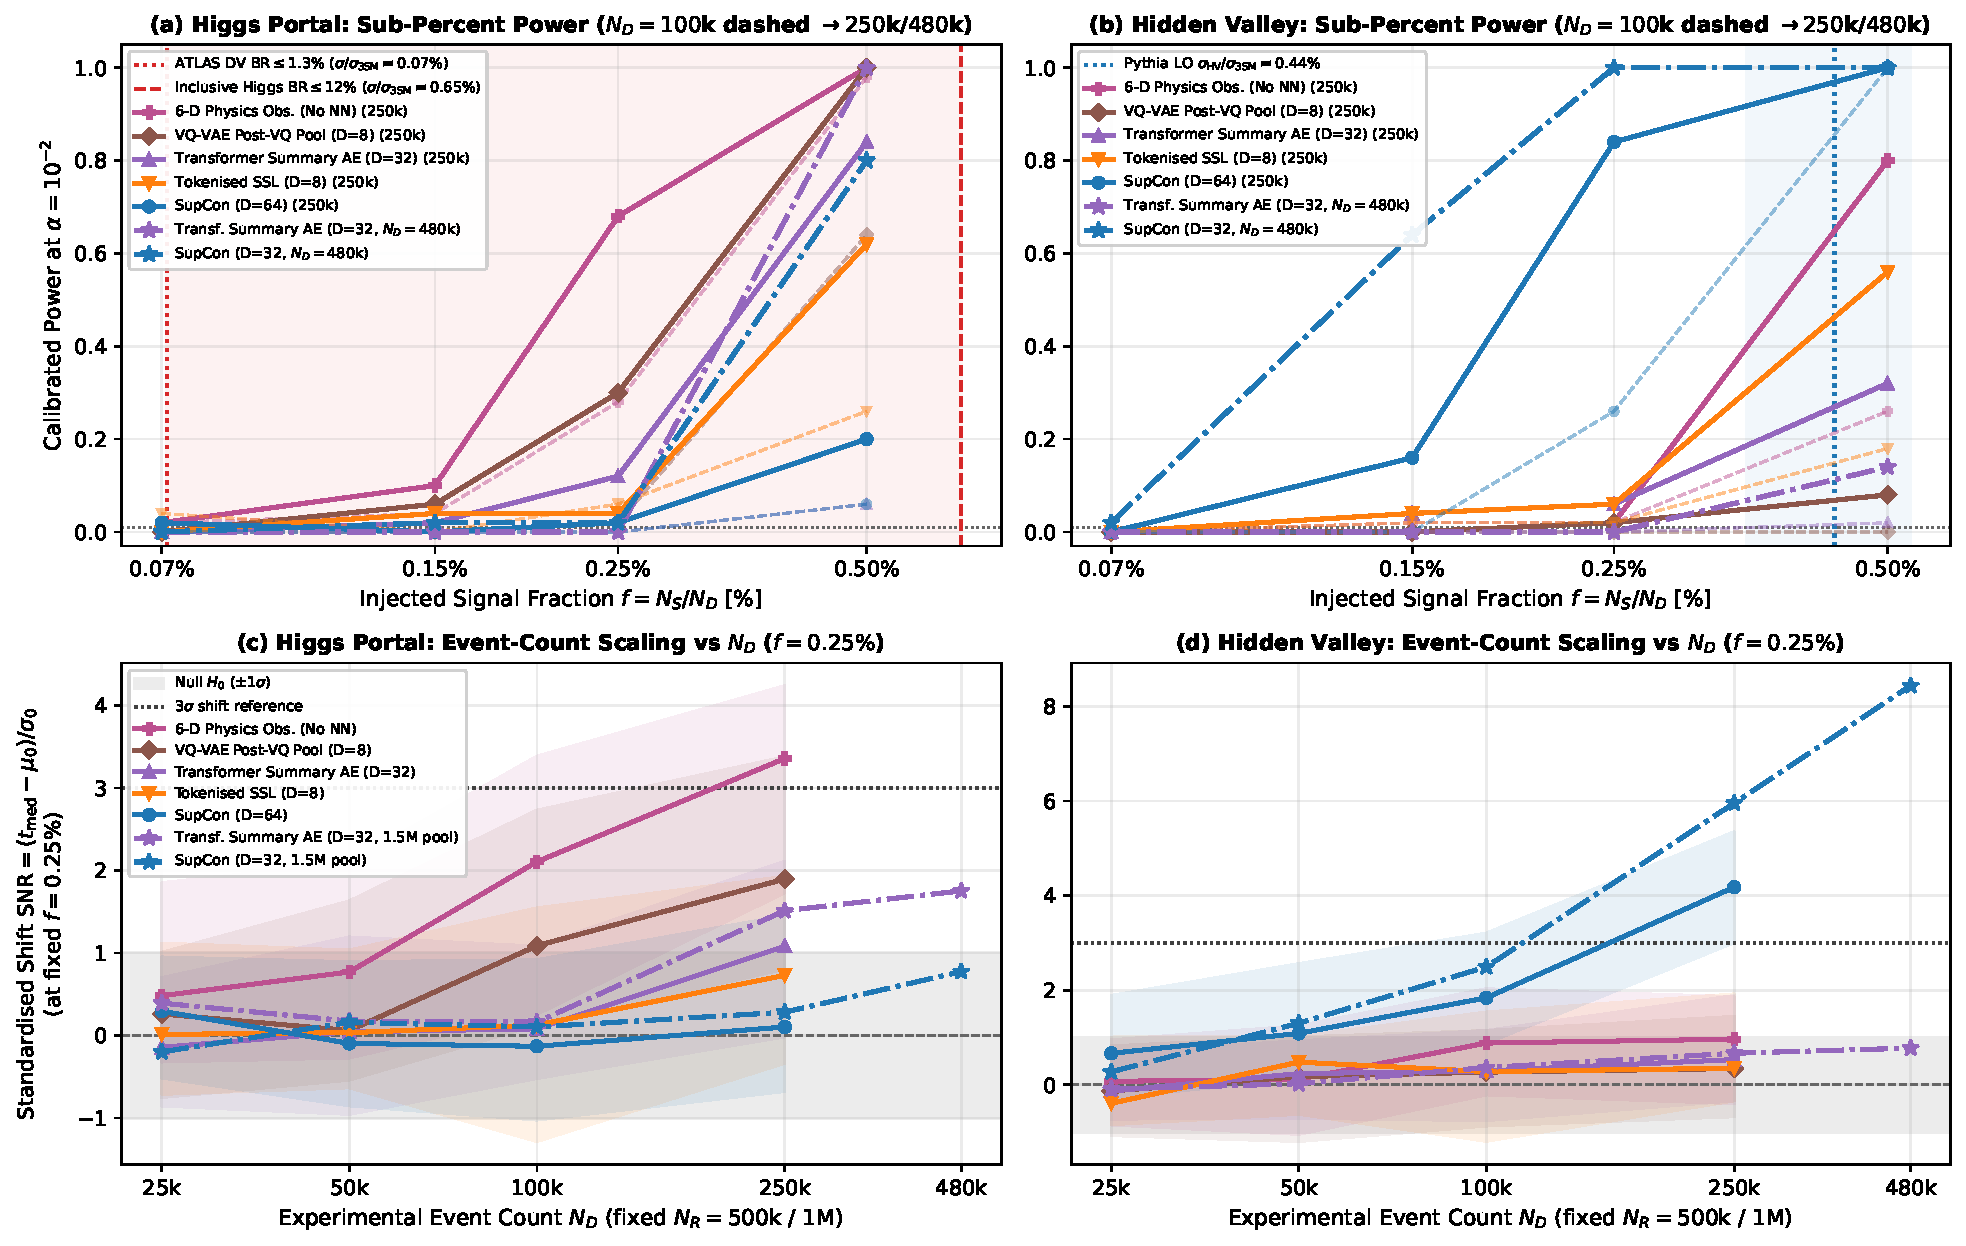
\includegraphics[width=0.97\textwidth]{fig_exclusion_and_nd_scaling.pdf}
    \caption{Sub-percent Kernel NPLM power and event-count scaling under joint $(\mathcal{R}, \mathcal{D})$ calibration ($M=1,000$ centres, median pairwise $\sigma$, $150$ calibration nulls plus $50$ validation nulls and $50$ signal toys per point). Panels (a) and (b) compare calibrated power at $\alpha = 10^{-2}$ for $N_D = 100\text{k}$ (dashed) against $N_D = 250\text{k}$ (solid, $N_R = 500\text{k}$) and $N_D = 480\text{k}$ (dash-dotted stars, $N_R = 1\text{M}$ on a $1.5\text{M}$-event SM pool), with three-process cross-section ratios $\sigma_S / \sigma_{\text{3SM}}$ overlaid as vertical reference lines. Panels (c) and (d) show median test-statistic shift $\text{SNR}$ ($[q_{16}, q_{84}]$ bands) versus experimental sample size $N_D \in \{25\text{k}, 50\text{k}, 100\text{k}, 250\text{k}, 480\text{k}\}$ at fixed $f = 0.25\%$.}
    \label{fig:exclusion_scaling}
}
\end{figure}

\section{Conclusion and Outlook}
\label{sec:conclusion}

Holding a Pre-LN Set Transformer architecture fixed across paradigms on $1.85\times 10^6$ zero-pileup ColliderML events, we have evaluated continuous contrastive learning, event-summary autoencoders, and discrete contextual VQ-VAE track tokenisation across supervised probes, low-label fine-tuning, and calibrated Kernel NPLM anomaly detection:
\begin{enumerate}
    \item \emph{Self-supervised track representations and discrete tokenisation.} Kinematically consistent spherical perigee augmentations (\texttt{ssl\_kinematic}) and discrete $K=8192$ tokenised contrastive pretraining (\texttt{ssl\_tokens}) reach $68.0\%$ and $68.9\%$ three-class SM linear accuracy at $D=64$, outperforming deterministic track summaries on linear classification and substantially improving low-label accuracy and stability at $N_{\text{labelled}} \le 10^3$ when paired with LP-FT fine-tuning. Despite training exclusively on prompt-dominated SM tracks, the contextual VQ-VAE preserves $97.5\%$ recall on reconstructed displaced tracks with $|d_0| > 1\text{ mm}$ without quantisation degradation.
    \item \emph{Task-metric trade-off in signal-agnostic anomaly detection.} Optimising an encoder for SM class separation compresses SM variance into a low-rank subspace ($\text{erank}_{\text{SM}} \le 3.5$), maximising Hidden Valley dark-shower sensitivity ($\text{SNR}_{1\%} = 35.0$) while forfeiting extreme low-FPR tail recall ($\text{FPR} \le 10^{-3}$) on displaced Higgs Portal decays that populate inter-class regions. Under isotropic Euclidean kernels, compact tail-preserving spaces ($D=8$ VQ-VAE poolings and the six-observable \texttt{phys\_handcrafted\_d6} baseline) yield two- to eightfold higher displaced-signal sensitivity, while \texttt{ssl\_tokens\_d8} and $D=32$ summary autoencoders provide the most balanced neural performance across both topologies.
    \item \emph{Sub-percent scaling and collider context.} Extending calibrated testing to $N_D = 250\text{k}$ and $480\text{k}$ yields high discovery power down to $f = 0.15\%$ to $0.50\%$, leaving an order-of-magnitude sensitivity gap relative to dedicated background-free displaced-vertex searches that narrows systematically with sample size when $N_R \gg N_D$.
\end{enumerate}

Three extensions follow naturally: extending full-event track tokenisers and anomaly benchmarks to High-Luminosity LHC pileup ($\langle\mu\rangle = 200$) with calorimeter and vertex objects, combining multi-bandwidth kernel aggregation~\cite{GrossoLetizia2024} with hybrid embeddings that concatenate learned event representations and compact displaced-track tail observables, and evaluating cross-section-weighted trigger streams alongside compute- and carbon-footprint accounting across pretraining and calibration stages.

\bibliographystyle{unsrt}
\bibliography{references}

\clearpage
\appendix

\section{Unified Architecture, Contextual Tokeniser, and Baseline Specifications}
\label{app:arch}

\paragraph{Unified Pre-LN Set Transformer.}
All set-level neural encoders map valid standardized tracks via a linear layer into $d_{\text{model}} = 64$, prepend a learnable $\texttt{[CLS]}$ token without positional encodings, and apply $L = 8$ Pre-LN Transformer encoder layers~\cite{PreLNTransformer} ($H = 8$ attention heads, feed-forward width $256$, GELU activations, dropout $0.025$) with key-padding masks on padded track slots. An output LayerNorm and linear projection map the final $\texttt{[CLS]}$ state to $\mathbf{z}_i \in \mathbb{R}^D$ ($D \in \{8, 32, 64\}$). Unified Pre-LN Set Transformers (\texttt{ssl\_kinematic}, \texttt{ssl\_tokens}, \texttt{ae\_transformer}, \texttt{supervised\_e2e}, \texttt{supervised\_scratch}, \texttt{random\_init}) use sequence cap $T = 128$ (20 cosine-annealed epochs for continuous models; 12 epochs for \texttt{ssl\_tokens}), while the \texttt{supcon} reference checkpoints use the identical parameterisation evaluated at $T = 256$ with dropout views ($\tau = 0.1$).

\paragraph{Contextual VQ-VAE track tokeniser and fidelity.}
In Eq.~\eqref{eq:track_vq6}, $p_T$ is floored at $10^{-3}\text{ GeV}$ and $\theta/2$ is clipped to $[10^{-6}, \pi/2 - 10^{-6}]$ before computing $\eta$. The contextual VQ-VAE ($T_{\text{VQ}} = 128$) uses a symmetric four-layer, eight-head Transformer encoder and decoder ($d_{\text{model}} = 128$, feed-forward width $512$), projecting valid track states to $\mathbf{z}_{e,ij} \in \mathbb{R}^8$ against an $8192$-code codebook ($\beta = 0.25$, exponential-moving-average updates with dead-code revival, and $2\times$ MSE weight on $\text{symlog}(d_0)$ and $\text{symlog}(z_0)$). Track- and event-level reconstruction fidelity on $2,656,735$ held-out SM tracks is shown in Fig.~\ref{fig:vqvae_fidelity}.

\paragraph{Two-stage LP-FT fine-tuning.}
For \texttt{ssl\_kinematic\_ft\_d64} and \texttt{ssl\_tokens\_ft\_d64}, track scalers are fit solely on the $80\%$ training portion of each labelled SM budget $N_{\text{labelled}} \in \{100, 10^3, 10^4, 10^5\}$. Five epochs of frozen-backbone linear-head warmup ($\text{lr} = 10^{-3}$) are followed by unfrozen fine-tuning ($\text{lr} = 2\times 10^{-4}$ on the Set Transformer and token embeddings, $10^{-3}$ on the head, conditioning on frozen VQ-VAE token indices).

\begin{figure}[htbp]
    \centering
    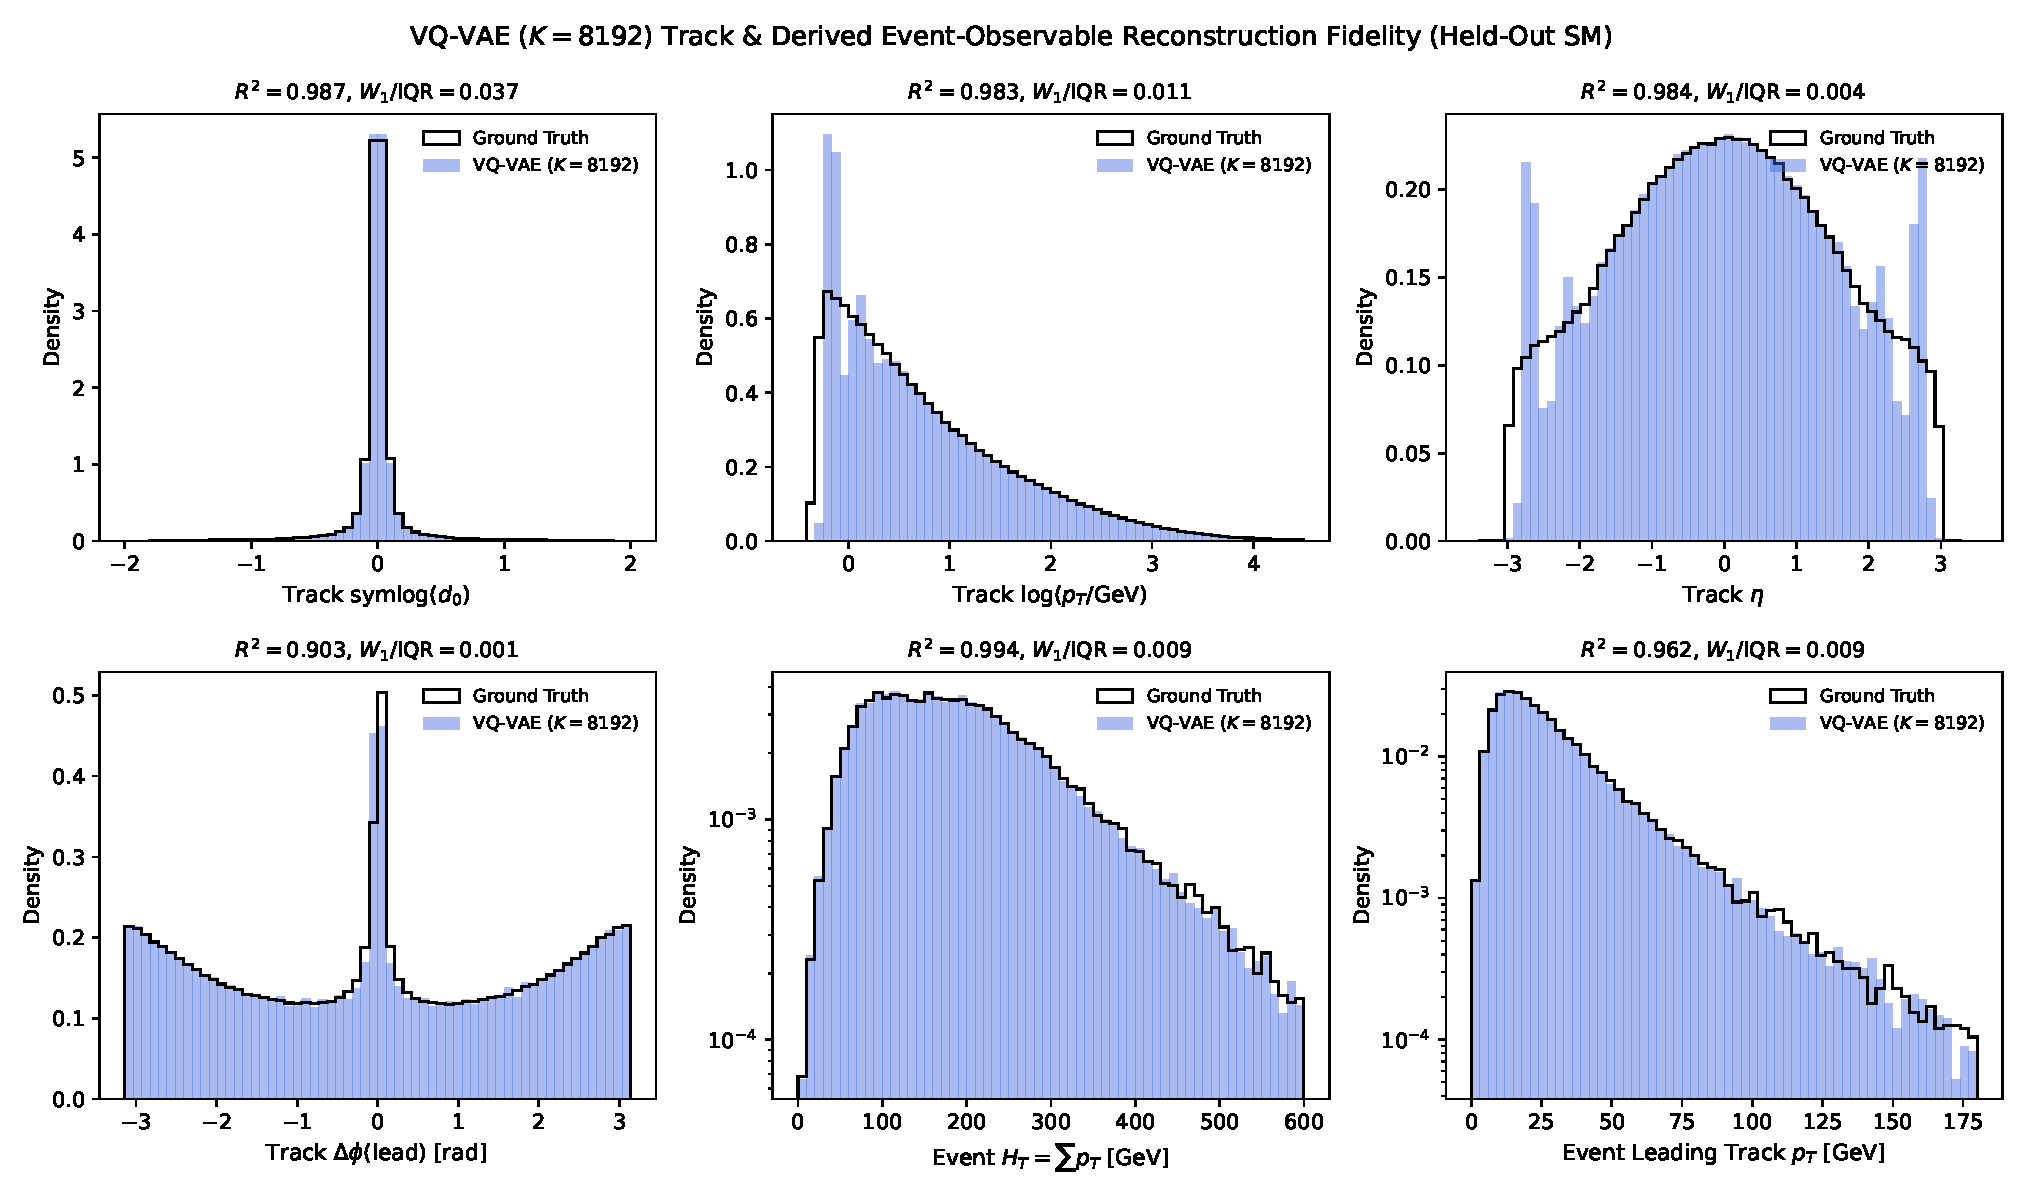
\includegraphics[width=0.96\textwidth]{fig_vqvae_fidelity.pdf}
    \caption{Track-level and event-level reconstruction fidelity of the $K=8192$ contextual VQ-VAE tokeniser across $2,656,735$ held-out SM tracks: (a to d) input versus quantised per-track coordinates, and (e to h) derived composite event observables ($H_T$, leading track $p_T$, $|\vec{p}_T^{\text{miss}}|$, and event $\text{RMS}(d_0)$).}
    \label{fig:vqvae_fidelity}
\end{figure}

\section{Full Downstream Classification and Transfer Probe Benchmarks}
\label{app:probes}

Table~\ref{tab:probes} reports paired classification and supervised BSM transfer probe metrics across all 27 primary representations on the $950,000$-event held-out evaluation split ($70\%$ train, $10\%$ validation, $20\%$ test; binary BSM transfer probes combine a fixed $60,000$-event balanced SM subset with $100,000$ signal events using inverse-frequency class weights). Table~\ref{tab:seed_lpft} reports three-seed pretraining reproducibility at $D=64$ alongside paired five-draw low-label SM-3 classification accuracy.

\begin{table}[htbp]
\centering
\caption{Paired downstream classification and supervised BSM transfer probes across all 27 primary representations. Bootstrap standard errors are $\le 0.0013$ on SM-3 accuracy and $\le 0.0009$ on transfer AUCs. Within each neural dimension $D \in \{8, 32, 64, 128\}$ and within the zero-network block, the highest unsupervised or self-supervised value per column is bolded.}
\label{tab:probes}
\resizebox{\linewidth}{!}{%
\begin{tabular}{llccccccccc}
\toprule
\textbf{Family / Model} & $D$ & $\text{erank}_{\text{SM}}$ & \textbf{SM-3 Lin Acc} & \textbf{SM-3 Lin AUC} & \textbf{SM-3 MLP Acc} & \textbf{SM-3 MLP AUC} & \textbf{5-Class Acc} & \textbf{5-Class AUC} & \textbf{Transfer HP} & \textbf{Transfer HV} \\
\midrule
\multicolumn{11}{l}{\textit{Supervised Reference Models (pretrained with SM class labels)}} \\
\texttt{supcon\_d8} & 8 & 2.58 & 0.8141 & 0.9393 & 0.8147 & 0.9400 & 0.6446 & 0.9174 & 0.8827 & 0.9309 \\
\texttt{supcon\_d32} & 32 & 3.21 & 0.8167 & 0.9405 & 0.8170 & 0.9409 & 0.7434 & 0.9450 & 0.9344 & 0.9899 \\
\texttt{supcon\_d64} & 64 & 3.50 & 0.8172 & 0.9409 & 0.8174 & 0.9416 & 0.7544 & 0.9472 & 0.9414 & 0.9895 \\
\texttt{supervised\_e2e\_d64}$^\dagger$ & 64 & 2.00 & 0.8153 & 0.9402 & 0.8147 & 0.9402 & 0.7495 & 0.9474 & 0.9348 & 0.9908 \\
\midrule
\multicolumn{11}{l}{\textit{Self-Supervised Contrastive (Pre-LN Set Transformer Backbone, Unlabelled SM Pretraining)}} \\
\texttt{ssl\_kinematic\_d8} & 8 & 5.82 & 0.6031 & 0.7823 & 0.6373 & 0.8085 & 0.4541 & 0.8213 & 0.8670 & 0.9068 \\
\texttt{ssl\_kinematic\_d32} & 32 & 8.57 & 0.6780 & 0.8415 & 0.6974 & 0.8554 & 0.5543 & 0.8660 & 0.9018 & 0.9300 \\
\texttt{ssl\_kinematic\_d64} & 64 & 8.30 & 0.6800 & 0.8421 & 0.7000 & 0.8569 & 0.5535 & 0.8669 & 0.8967 & 0.9307 \\
\texttt{ssl\_kinematic\_drop\_d64} & 64 & 14.36 & 0.6760 & 0.8375 & 0.7230 & 0.8724 & 0.5556 & 0.8614 & 0.8946 & 0.9253 \\
\texttt{ssl\_tokens\_d8} & 8 & 3.37 & \textbf{0.6439} & \textbf{0.8158} & \textbf{0.6622} & \textbf{0.8299} & \textbf{0.5250} & \textbf{0.8452} & 0.8805 & \textbf{0.9227} \\
\texttt{ssl\_tokens\_d32} & 32 & 8.44 & \textbf{0.6797} & \textbf{0.8435} & 0.6962 & 0.8582 & 0.5711 & 0.8688 & 0.9001 & 0.9322 \\
\texttt{ssl\_tokens\_d64} & 64 & 9.20 & \textbf{0.6893} & \textbf{0.8496} & 0.7035 & 0.8632 & 0.5854 & 0.8749 & 0.9023 & 0.9413 \\
\midrule
\multicolumn{11}{l}{\textit{Unsupervised 28-D Physics Summary Bottlenecks (Unlabelled SM Pretraining)}} \\
\texttt{ae\_transformer\_d8} & 8 & 3.37 & 0.4706 & 0.6526 & 0.6132 & 0.7892 & 0.3599 & 0.7210 & 0.7704 & 0.8521 \\
\texttt{ae\_transformer\_d32} & 32 & 16.65 & 0.6618 & 0.8280 & \textbf{0.7236} & \textbf{0.8743} & \textbf{0.5909} & \textbf{0.8714} & 0.9087 & \textbf{0.9603} \\
\texttt{ae\_transformer\_d64} & 64 & 16.95 & 0.6832 & 0.8431 & \textbf{0.7284} & \textbf{0.8786} & \textbf{0.6173} & \textbf{0.8838} & 0.9235 & \textbf{0.9611} \\
\texttt{ae\_mlp\_d8} & 8 & 7.16 & 0.5585 & 0.7261 & 0.6014 & 0.7751 & 0.4437 & 0.7837 & 0.8014 & 0.9175 \\
\texttt{ae\_mlp\_d32} & 32 & 16.00 & 0.6557 & 0.8225 & 0.7146 & 0.8684 & 0.5887 & 0.8711 & \textbf{0.9275} & 0.9586 \\
\texttt{ae\_mlp\_d64} & 64 & 17.18 & 0.6594 & 0.8261 & 0.7159 & 0.8696 & 0.5980 & 0.8761 & \textbf{0.9301} & 0.9603 \\
\midrule
\multicolumn{11}{l}{\textit{Frozen Contextual VQ-VAE Poolings and Untrained Random Baselines}} \\
\texttt{vqvae\_code\_d8} (pure pre-VQ $\mathbf{z}_e$) & 8 & 5.35 & 0.5596 & 0.7449 & 0.6021 & 0.7837 & 0.4341 & 0.7973 & 0.9097 & 0.8260 \\
\texttt{vqvae\_quant\_d8} (pure post-VQ $\mathbf{z}_q$) & 8 & 5.32 & 0.5592 & 0.7446 & 0.5998 & 0.7816 & 0.4355 & 0.7981 & \textbf{0.9118} & 0.8273 \\
\texttt{vqvae\_encoder\_d128} & 128 & 8.46 & \textbf{0.7007} & \textbf{0.8586} & \textbf{0.7437} & \textbf{0.8915} & \textbf{0.6642} & \textbf{0.9069} & \textbf{0.9549} & \textbf{0.9774} \\
\texttt{random\_init\_d8} & 8 & 1.90 & 0.5083 & 0.6893 & 0.5951 & 0.7727 & 0.3565 & 0.7496 & 0.7788 & 0.8765 \\
\texttt{random\_init\_d32} & 32 & 2.97 & 0.5872 & 0.7689 & 0.6665 & 0.8293 & 0.4488 & 0.8097 & 0.8393 & 0.9047 \\
\texttt{random\_init\_d64} & 64 & 2.75 & 0.6236 & 0.7963 & 0.6857 & 0.8446 & 0.5206 & 0.8427 & 0.8923 & 0.9298 \\
\midrule
\multicolumn{11}{l}{\textit{Zero-Network Physics Baselines (Deterministic Summaries and Classical Observables)}} \\
\texttt{raw\_summary\_d28} (28-D summary) & 28 & 16.59 & 0.6413 & 0.8132 & \textbf{0.7117} & \textbf{0.8662} & 0.5643 & 0.8614 & 0.9125 & \textbf{0.9545} \\
\texttt{pca\_summary\_d8} (top-8 SM PCA) & 8 & 7.90 & 0.5603 & 0.7426 & 0.6473 & 0.8191 & 0.4411 & 0.7978 & 0.8799 & 0.9261 \\
\texttt{phys\_handcrafted\_d6} (6-D obs.) & 6 & 3.46 & \textbf{0.6747} & \textbf{0.8383} & 0.7003 & 0.8570 & \textbf{0.5904} & \textbf{0.8784} & \textbf{0.9296} & 0.9446 \\
\texttt{mult\_only\_d1} ($N_{\text{tracks}}$ only) & 1 & 1.00 & 0.4846 & 0.6749 & 0.4927 & 0.6799 & 0.2882 & 0.7032 & 0.7508 & 0.7418 \\
\bottomrule
\multicolumn{11}{l}{\footnotesize $^\dagger$Direct end-to-end head on \texttt{supervised\_e2e\_d64} yields $0.8131$ SM-3 accuracy and $0.9398$ ROC-AUC.}
\end{tabular}%
}
\end{table}

\begin{table}[htbp]
\centering
\caption{(A) Three-seed pretraining variability at $D=64$ ($250$-null NPLM protocol). (B) Paired five-draw SM-3 classification accuracy across label budgets $N_{\text{labelled}}$ (mean $\pm$ SD).}
\label{tab:seed_lpft}
\resizebox{\linewidth}{!}{%
\begin{tabular}{llcccc}
\toprule
\multicolumn{6}{l}{\textbf{(A) Three-Seed Pretraining Reproducibility at $D=64$}} \\
\textbf{Configuration} & \textbf{Protocol} & \textbf{SM-3 Lin Acc} & \textbf{Transfer HP AUC} & \textbf{1\% HP SNR} & \textbf{1\% HV SNR} \\
\midrule
\texttt{ssl\_kinematic\_d64} & Pre-LN $T=128$ kinematic SSL (3 seeds) & $0.6790 \pm 0.0019$ & $0.8930 \pm 0.0060$ & $3.50 \pm 0.45$ & $3.87 \pm 0.18$ \\
\texttt{ssl\_tokens\_d64} & Pre-LN $T=128$ tokenised SSL (3 seeds)$^\S$ & $0.6858 \pm 0.0079$ & $0.9039 \pm 0.0026$ & $4.62 \pm 0.25$ & $5.31 \pm 0.85$ \\
\midrule
\multicolumn{6}{l}{\textbf{(B) Paired Five-Draw SM-3 Classification Accuracy Across Label Budgets (Mean $\pm$ SD)}} \\
\textbf{Model / Regime} & \textbf{Head / Adaptation} & $N_{\text{labelled}}=100$ & $N_{\text{labelled}}=10^3$ & $N_{\text{labelled}}=10^4$ & $N_{\text{labelled}}=10^5$ \\
\midrule
\texttt{supervised\_scratch\_d64} & End-to-end from random init & $0.5228 \pm 0.0721$ & $0.6518 \pm 0.0279$ & $0.7190 \pm 0.0056$ & $0.7608 \pm 0.0024$ \\
\texttt{ssl\_kinematic\_d64} & Frozen encoder + linear probe & $0.5401 \pm 0.1021$ & $0.6475 \pm 0.0027$ & $0.6673 \pm 0.0006$ & $0.6762 \pm 0.0004$ \\
\texttt{ssl\_kinematic\_ft\_d64} & Pretrained + LP-FT unfrozen & $0.6124 \pm 0.0340$ & $0.6782 \pm 0.0048$ & $0.7126 \pm 0.0023$ & $0.7451 \pm 0.0004$ \\
\texttt{ssl\_tokens\_d64} & Frozen encoder + linear probe & $0.5853 \pm 0.0290$ & $0.6621 \pm 0.0042$ & $0.6769 \pm 0.0022$ & $0.6862 \pm 0.0003$ \\
\texttt{ssl\_tokens\_ft\_d64} & Pretrained + LP-FT token enc.$^\S$ & $0.5865 \pm 0.0269$ & $0.6738 \pm 0.0063$ & $0.7066 \pm 0.0024$ & $0.7323 \pm 0.0007$ \\
\bottomrule
\multicolumn{6}{l}{\footnotesize $^\S$Tokenised SSL seed and fine-tuning runs condition on the fixed SM-pretrained $K=8192$ VQ-VAE tokeniser.}
\end{tabular}%
}
\end{table}

\section{Kernel NPLM Solver, Calibration Diagnostics, and ROC-Tail Controls}
\label{app:nplm}

\paragraph{GPU Newton-Raphson solver and rate-versus-shape check.}
Because Nystr\"om kernel matrices $K_{MM}$ exhibit condition numbers near $10^8$, quasi-Newton L-BFGS requires $\sim 21.5\text{ s}$ per toy at $N_R = 500\text{k}$. Precomputing the $(N, M)$ kernel feature matrix on GPU and assembling the exact gradient and $M\times M$ Hessian in \texttt{float64} with damped backtracking line search converges in four to five Newton steps ($\sim 30\text{ ms}$ per toy at $M=316$). Under additive injection ($N_D = N_B + N_S$), a constant log-intensity shift $f_0 = \log(N_D / N_B)$ produces
\begin{equation}
    t_{\text{rate}}(N_B, N_S) = 2\left[(N_B + N_S)\log\!\left(1 + \frac{N_S}{N_B}\right) - N_S\right] \approx \frac{N_S^2}{N_B} ,
    \label{eq:t_rate}
\end{equation}
reaching $245.9$ at $5\%$ injection (Fig.~\ref{fig:nplm_cal}b), whereas fixed-size shape-only mixtures ($N_D = N_B = 100\text{k}$) enforce $t_{\text{rate}} \equiv 0$. Out-of-sample validation false-positive rates across the 16 models in Table~\ref{tab:nplm_highstats} lie in $[0.0078, 0.0132]$ at $\alpha = 10^{-2}$ and $[0.0000, 0.0020]$ at $\alpha = 10^{-3}$. Model orderings are invariant under both a low-overlap check ($N_R = 350\text{k}$, $N_{\text{pool}} = 400\text{k}$, $N_B = 25\text{k}$) and five independent draws of $\mathcal{R}$ and kernel centres ($\text{SNR}_{1\%} = 27.3 \pm 2.5$ for \texttt{phys\_handcrafted\_d6}, $17.9 \pm 1.9$ for \texttt{vqvae\_quant\_d8}, and $4.3 \pm 0.6$ for \texttt{supcon\_d64}). Table~\ref{tab:nplm} presents the complete 27-model sweep, and Table~\ref{tab:roc_tail} reports the extreme-tail supervised ROC crossover alongside bandwidth and ZCA ablations.

\begin{figure}[htbp]
    \centering
    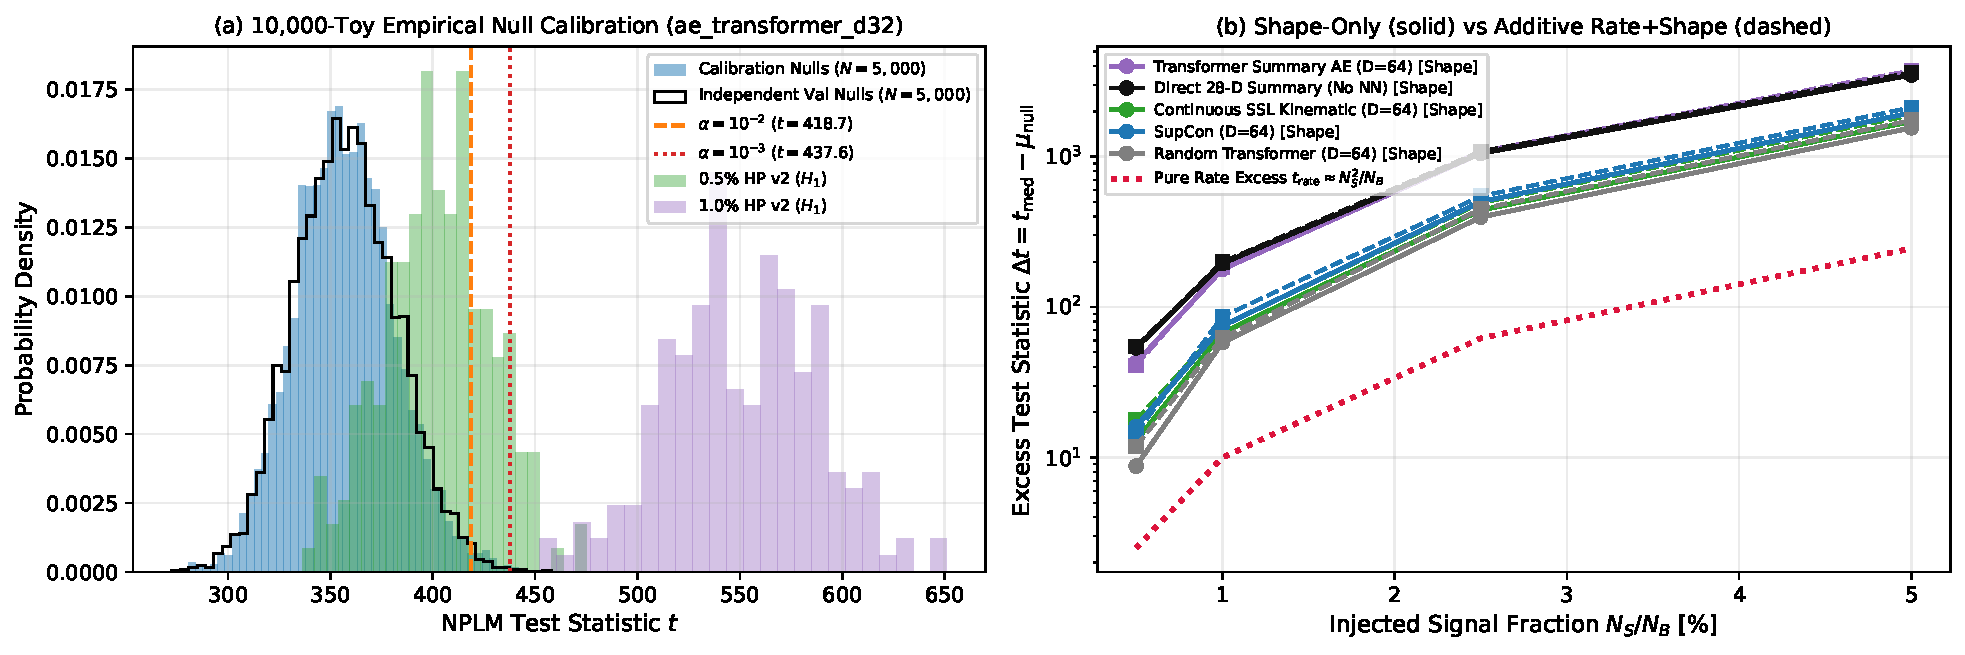
\includegraphics[width=0.96\textwidth]{fig_nplm_calibration_and_rate.pdf}
    \caption{Conditional null calibration and rate-versus-shape separation in Kernel NPLM: (a) $5,000$ calibration nulls versus $5,000$ independent validation nulls for \texttt{ae\_transformer\_d32} alongside $0.5\%$ and $1.0\%$ Higgs Portal toys; (b) fixed-size shape-only mixtures ($N_D = N_B = 100\text{k}$, solid) versus additive injection ($N_D = N_B + N_S$, dashed) and pure Poisson rate excess $t_{\text{rate}}$ (dotted red).}
    \label{fig:nplm_cal}
\end{figure}

\begin{table}[htbp]
\centering
\caption{Paired shape-only Kernel NPLM sweep across all 27 primary representations ($N_R=500\text{k}$, $N_D=100\text{k}$, $M=316$, $q=0.90$, $250$ paired nulls, $100$ paired signal toys per point). Top neural and zero-network values per column are bolded.}
\label{tab:nplm}
\resizebox{\linewidth}{!}{%
\begin{tabular}{llcc|ccccc|ccccc}
\toprule
& & \multicolumn{2}{c|}{\textbf{Null ($250$)}} & \multicolumn{5}{c|}{\textbf{Higgs Portal (Displaced LLP)}} & \multicolumn{5}{c}{\textbf{Hidden Valley (Dark Shower)}} \\
\textbf{Model} & $D$ & $\mu_{\text{null}}$ & $\sigma_{\text{null}}$ & \textbf{SNR 0.5\%} & \textbf{SNR 1.0\%} & $\textbf{Pow}_{10^{-2}}$ & $Z_{\text{asym}}$ & \textbf{SNR 2.5\%} & \textbf{SNR 0.5\%} & \textbf{SNR 1.0\%} & $\textbf{Pow}_{10^{-2}}$ & $Z_{\text{asym}}$ & \textbf{SNR 2.5\%} \\
\midrule
\multicolumn{14}{l}{\textit{Supervised Reference Models (pretrained with SM class labels)}} \\
\texttt{supcon\_d8} & 8 & 90.1 & 11.6 & 0.65 & 3.44 & 0.76 & 3.06 & 21.7 & 3.01 & 13.00 & \textbf{1.00} & 9.13 & 74.9 \\
\texttt{supcon\_d32} & 32 & 242.8 & 19.2 & 0.90 & 3.99 & 0.86 & 3.67 & 23.9 & 8.33 & \textbf{33.68} & \textbf{1.00} & \textbf{20.96} & \textbf{169.3} \\
\texttt{supcon\_d64} & 64 & 287.7 & 22.3 & 0.72 & 3.36 & 0.57 & 3.15 & 22.6 & \textbf{9.09} & 32.40 & \textbf{1.00} & 20.61 & 157.3 \\
\texttt{supervised\_e2e\_d64} & 64 & 353.0 & 24.1 & 0.39 & 2.27 & 0.56 & 2.18 & 17.9 & 3.50 & 14.68 & \textbf{1.00} & 11.49 & 83.2 \\
\midrule
\multicolumn{14}{l}{\textit{Self-Supervised Contrastive (Pre-LN Set Transformer Backbone)}} \\
\texttt{ssl\_kinematic\_d8} & 8 & 115.7 & 12.6 & 0.75 & 4.34 & 0.94 & 3.79 & 27.3 & 1.07 & 4.64 & 0.96 & 4.02 & 25.9 \\
\texttt{ssl\_kinematic\_d32} & 32 & 226.3 & 18.1 & 1.11 & 4.36 & 0.90 & 3.94 & 27.4 & 0.99 & 4.30 & 0.93 & 3.90 & 25.4 \\
\texttt{ssl\_kinematic\_d64} & 64 & 224.6 & 18.6 & 0.69 & 3.63 & 0.70 & 3.34 & 23.7 & 0.98 & 3.93 & 0.83 & 3.59 & 24.1 \\
\texttt{ssl\_kinematic\_drop\_d64} & 64 & 339.4 & 23.4 & 0.20 & 2.62 & 0.30 & 2.52 & 17.0 & 0.79 & 2.78 & 0.38 & 2.66 & 17.4 \\
\texttt{ssl\_tokens\_d8} & 8 & 55.3 & 9.6 & 1.42 & 5.91 & 0.98 & 4.66 & 36.3 & 1.61 & 6.48 & \textbf{1.00} & 5.01 & 38.4 \\
\texttt{ssl\_tokens\_d32} & 32 & 226.1 & 18.2 & 1.22 & 4.47 & 0.87 & 4.04 & 27.9 & 1.18 & 4.84 & 0.95 & 4.33 & 28.2 \\
\texttt{ssl\_tokens\_d64} & 64 & 263.6 & 18.4 & 1.30 & 4.88 & 0.97 & 4.44 & 28.9 & 1.45 & 5.13 & \textbf{1.00} & 4.65 & 30.3 \\
\midrule
\multicolumn{14}{l}{\textit{Unsupervised 28-D Physics Summary Bottlenecks}} \\
\texttt{ae\_transformer\_d8} & 8 & 162.5 & 16.0 & 2.16 & 8.09 & \textbf{1.00} & 6.64 & 45.4 & 0.90 & 4.03 & 0.90 & 3.64 & 21.5 \\
\texttt{ae\_transformer\_d32} & 32 & 357.9 & 24.8 & 2.11 & 7.65 & \textbf{1.00} & 6.63 & 43.8 & 1.50 & 6.24 & \textbf{1.00} & 5.55 & 35.3 \\
\texttt{ae\_transformer\_d64} & 64 & 354.7 & 24.4 & 1.74 & 7.29 & \textbf{1.00} & 6.36 & 43.1 & 1.76 & 6.77 & \textbf{1.00} & 5.96 & 36.7 \\
\texttt{ae\_mlp\_d8} & 8 & 196.8 & 17.4 & 2.62 & 8.72 & \textbf{1.00} & 7.22 & 44.3 & 1.00 & 3.55 & 0.82 & 3.29 & 20.3 \\
\texttt{ae\_mlp\_d32} & 32 & 361.0 & 26.8 & 2.01 & 7.44 & \textbf{1.00} & 6.41 & 40.2 & 0.97 & 4.32 & 0.95 & 3.95 & 24.1 \\
\texttt{ae\_mlp\_d64} & 64 & 357.9 & 24.7 & 1.98 & 7.45 & \textbf{1.00} & 6.48 & 41.0 & 0.91 & 4.41 & 0.96 & 4.05 & 26.1 \\
\midrule
\multicolumn{14}{l}{\textit{Frozen Contextual VQ-VAE Poolings and Untrained Random Baselines}} \\
\texttt{vqvae\_code\_d8} (pure $\mathbf{z}_e$) & 8 & 177.6 & 15.1 & 4.71 & 18.28 & \textbf{1.00} & 13.02 & 89.5 & 0.01 & 1.90 & 0.32 & 1.83 & 11.2 \\
\texttt{vqvae\_quant\_d8} (pure $\mathbf{z}_q$) & 8 & 179.8 & 15.1 & \textbf{4.92} & \textbf{18.41} & \textbf{1.00} & \textbf{13.20} & \textbf{90.6} & 0.09 & 1.75 & 0.22 & 1.70 & 11.2 \\
\texttt{vqvae\_encoder\_d128} & 128 & 321.1 & 22.4 & 1.04 & 7.23 & \textbf{1.00} & 6.33 & 45.9 & 1.30 & 5.61 & \textbf{1.00} & 5.06 & 33.2 \\
\texttt{random\_init\_d8} & 8 & 107.6 & 12.9 & -0.04 & 1.53 & 0.13 & 1.47 & 12.5 & 1.45 & 4.25 & 0.93 & 3.68 & 25.1 \\
\texttt{random\_init\_d32} & 32 & 194.9 & 15.4 & 0.74 & 3.14 & 0.69 & 2.95 & 21.8 & 1.60 & 5.09 & 0.92 & 4.57 & 25.8 \\
\texttt{random\_init\_d64} & 64 & 164.7 & 14.5 & 0.60 & 4.01 & 0.85 & 3.63 & 27.4 & 1.55 & 5.30 & 0.99 & 4.66 & 28.7 \\
\midrule
\multicolumn{14}{l}{\textit{Zero-Network Physics Baselines (Deterministic Summaries and Classical Observables)}} \\
\texttt{raw\_summary\_d28} (28-D summary) & 28 & 333.9 & 24.1 & 2.22 & 8.09 & \textbf{1.00} & 6.91 & 43.6 & 1.20 & 5.12 & 0.97 & 4.61 & 27.8 \\
\texttt{pca\_summary\_d8} (top-8 PCA) & 8 & 209.1 & 17.9 & 2.59 & 9.19 & \textbf{1.00} & 7.56 & 47.8 & 0.81 & 3.48 & 0.63 & 3.23 & 17.9 \\
\texttt{phys\_handcrafted\_d6} (6-D obs.) & 6 & 91.4 & 12.0 & \textbf{8.91} & \textbf{28.42} & \textbf{1.00} & \textbf{15.93} & \textbf{134.7} & \textbf{2.18} & \textbf{8.63} & \textbf{1.00} & \textbf{6.64} & \textbf{50.2} \\
\texttt{mult\_only\_d1} ($N_{\text{tracks}}$ only) & 1 & 8.1 & 3.6 & 1.28 & 4.71 & 0.72 & 3.23 & 27.2 & -0.78 & 0.16 & 0.00 & 0.30 & 9.1 \\
\bottomrule
\end{tabular}%
}
\end{table}

\begin{table}[htbp]
\centering
\caption{Supervised binary linear probe ROC-tail recall at held-out SM $\text{FPR} \in \{10^{-1}, 10^{-3}, 10^{-4}\}$ ($702,000$ SM test events) versus $1\%$ Higgs Portal Kernel NPLM $\text{SNR}$ ($250$-null protocol) across kernel centres, bandwidth quantiles, and shrinkage ZCA whitening.}
\label{tab:roc_tail}
\resizebox{\linewidth}{!}{%
\begin{tabular}{lccccc}
\toprule
\textbf{Representation} & \textbf{Transfer AUC ($\text{TPR}@10^{-1}$)} & $\textbf{TPR}@\textbf{FPR}=10^{-3}$ & $\textbf{TPR}@\textbf{FPR}=10^{-4}$ & \textbf{NPLM SNR ($q=0.90$)} & \textbf{NPLM SNR ($q=0.25$ / ZCA)} \\
\midrule
\texttt{supcon\_d64} ($D=64$) & $0.9414$ ($0.8417$) & $0.0270$ & $0.0034$ & $3.36$ (PCs 1--3: $4.11$) & $2.86$ / $3.46$ \\
\texttt{ssl\_kinematic\_d64} ($D=64$) & $0.8967$ ($0.6841$) & $0.0435$ & $0.0080$ & $3.63$ ($M=1000$: $3.72$) & $2.92$ / $3.52$ \\
\texttt{ae\_transformer\_d32} ($D=32$) & $0.9088$ ($0.7355$) & $0.1281$ & $0.0325$ & $7.65$ ($M=1000$: $8.12$) & $5.21$ / $6.42$ \\
\texttt{vqvae\_quant\_d8} ($D=8$) & $0.9118$ ($0.7332$) & $0.1146$ & $0.0313$ & $18.41$ ($M=1000$: $19.00$) & $7.74$ / $16.89$ \\
\texttt{raw\_summary\_d28} ($D=28$) & $0.9124$ ($0.7547$) & $0.1402$ & $0.0411$ & $8.09$ ($M=1000$: $8.72$) & $4.72$ / $6.92$ \\
\texttt{phys\_handcrafted\_d6} ($D=6$) & $0.9297$ ($0.7816$) & $0.0792$ & $0.0122$ & $28.42$ ($M=1000$: $29.44$) & $16.69$ / $23.15$ \\
\bottomrule
\end{tabular}%
}
\end{table}

\section{Supplementary Low-Dimensional Embedding Sweep}
\label{app:lowd_sweep}

Figure~\ref{fig:classification_performance} shows exploratory classification accuracy and ROC-AUC across low bottleneck dimensions $D \in \{2, 4, 8, 16, 32\}$ evaluated on the $1.5\text{M}$-event SM pretraining split ($T = 500$ track cap) with displaced Higgs Portal events.

\begin{figure}[htbp]
    \centering
    \begin{subfigure}{0.48\textwidth}
        \centering
        \includegraphics[width=\linewidth]{Plots/acc_vs_d.png}
        \caption{Linear classification accuracy versus $D$.}
        \label{fig:acc_finalrun}
    \end{subfigure}
    \hfill
    \begin{subfigure}{0.48\textwidth}
        \centering
        \includegraphics[width=\linewidth]{Plots/auc_vs_d.png}
        \caption{Macro ROC-AUC versus $D$.}
        \label{fig:auc_finalrun}
    \end{subfigure}
    \caption{Exploratory low-dimensional linear probe scaling across $D \in \{2, 4, 8, 16, 32\}$ ($T = 500$, $1.5\text{M}$-event SM pretraining campaign).}
    \label{fig:classification_performance}
\end{figure}

\end{document}
